%% Customizações do abnTeX2 (http://www.abntex.net.br) para o Instituto de Matemática,
%% Estatística e Computação Científica da Universidade Estadual de Campinas (IMECC-UNICAMP)
%%
%% This work may be distributed and/or modified under the conditions of the LaTeX Project
%% Public License, either version 1.3 of this license or (at your option) any later version.
%% The latest version of this license is in http://www.latex-project.org/lppl.txt and version
%% 1.3 or later is part of all distributions of LaTeX version 2005/12/01 or later.
%%
%% This work has the LPPL maintenance status `maintained'.
%% 
%% The Current Maintainer of this work is Fábio Rodrigues Silva, gfabinhomat@gmail.com
%%
%% Further information about abnTeX2 are available on http://www.abntex.net.br
%%
\documentclass[
	oldfontcommands,
	% -- opções de customização --
	%sumario=tradicional,
	sumario=abnt-6027-2012,
	% -- opções da classe memoir --
	12pt,			% tamanho da fonte
	openright,		% capítulos começam em pág ímpar (insere página vazia caso preciso)
	oneside,		% para impressão em verso e anverso. Oposto a 'oneside'
	a4paper,		% tamanho do papel. 
	% -- opções da classe abntex2 --
	%chapter=TITLE,		% títulos de capítulos convertidos em letras maiúsculas
	%section=TITLE,		% títulos de seções convertidos em letras maiúsculas
	%subsection=TITLE,	% títulos de subseções convertidos em letras maiúsculas
	%subsubsection=TITLE,	% títulos de subsubseções convertidos em letras maiúsculas
	% -- opções do pacote babel --
	english,		% idioma adicional para hifenização
	brazil			% o último idioma é o principal do documento
	]{imecc-unicamp}
% ----------------------------------------------------------
% PACOTES ESSENCIAIS
% Aqui você pode adicionar seus pacotes específicos para uso em seu trabalho.
% Em PACOTES PESSOAIS insira os pacotes que desejar.
% ----------------------------------------------------------
% PACOTES BÁSICOS (ESSENCIAIS AO MODELO)
\usepackage{lmodern}			% Usa a fonte Latin Modern
\usepackage[T1]{fontenc}		% Selecao de codigos de fonte.
\usepackage[utf8]{inputenc}		% Codificacao do documento (conversão automática dos acentos)
\usepackage{lastpage}			% Usado pela Ficha catalográfica
\usepackage{indentfirst}		% Indenta o primeiro parágrafo de cada seção.
\usepackage{color,xcolor}		% Controle das cores
\usepackage{graphicx}			% Inclusão de gráficos
\usepackage{microtype} 			% para melhorias de justificação
% ----------------------------------------------------------
% ----------------------------------------------------------
% PACOTES PARA GLOSSÁRIO
\usepackage[subentrycounter,seeautonumberlist,nonumberlist=true]{glossaries}
% para usar o xindy ao invés do makeindex:
%\usepackage[xindy={language=portuguese},subentrycounter,seeautonumberlist,nonumberlist=true]{glossaries}
% ----------------------------------------------------------
% ----------------------------------------------------------
% PACOTES DE CITAÇÕES (PRINCIPAIS PACOTES DO MODELO)
\usepackage[brazilian]{backref}		% Paginas com as citações na bibl
\usepackage[alf,
	    abnt-repeated-author-omit=yes,
	    abnt-etal-list=0]{abntex2cite}		% Citações padrão ABNT
\makeatletter
\@ifpackageloaded{tocbibind}{}{\let\tocbibind\relax}
\makeatother

% É possível utilizar o sistema numérico de chamada, alterando a opção 'alf' para 'num'.
% Outros estilos bibliográficos podem ser usados. Se este for o caso, comente o pacote acima
% e utilize, por exemplo, o comando abaixo
% \bibliographystyle{acm}
% Consulte outros estilos de bibliografia consultando o manual de estilos bibliográficos do
% BibTeX em 'http://www.bibtex.org/'
% ----------------------------------------------------------
% ----------------------------------------------------------
% PACOTES ADICIONAIS (usados apenas no âmbito do Modelo Canônico do abnteX2)
\usepackage{lipsum}			% para geração de dummy text
% ----------------------------------------------------------
% ----------------------------------------------------------
% PACOTES PESSOAIS (USADOS PELO AUTOR -- acrescente aqui seus pacotes)
% ----------------------------------------------------------
\usepackage[portuguese,onelanguage]{algorithm2e}	% para inserir algoritmos (longend,vlined)
\usepackage{float}
% \usepackage{amsbsy}			% para símbolos matemáticos em negrito
% \usepackage{amscd}			% para diagramas
% \usepackage{amsfonts}			% fontes AMS
% \usepackage{amsmath}			% facilidades matemáticas
% \usepackage{amssymb}			% para os símbolos mais antigos
% \usepackage{amstext}			% para fragmentos tipo texto em modo matemático
\usepackage{amsthm}			% para teoremas
\usepackage{hyperref}			% Amplo suporte para hipertexto em LaTeX
\usepackage{cleveref}			% Referência cruzada inteligente
\usepackage{dsfont}			% para o estilo de conjuntos de números $\mathds{R}$
% \usepackage{ifthen}			% comandos de condição em LaTeX
\usepackage{listings}           	% para inserir códigos de outras linguagens de programação
% \usepackage{lscape}             	% para imprimir alguma página no formato paisagem
\usepackage{mathabx}			% conjunto de simbolos matemáticos
% \usepackage{mathrsfs}			% suporte para fontes RSFS
% \usepackage{pdfpages}           	% para inserir páginas PDF no texto

% \usepackage{verbatim}
% ----------------------------------------------------------
\usepackage{lastpage}
\usepackage{graphics}
\usepackage{float}
\usepackage{graphicx}
\usepackage{lscape}
\usepackage{longtable}
\usepackage{rotating}
\usepackage{graphics} 
\usepackage{ifthen}
\usepackage{keyval}
\usepackage{trig}
\usepackage{tabu}
\usepackage{varwidth}
% Indenta o primeiro parágrafo de cada seção.
\usepackage{indentfirst}
\usepackage{lscape}
\usepackage{array}
% Controle das cores.
\usepackage[usenames,dvipsnames]{xcolor}

% Inclusão de gráficos.
\usepackage{graphicx}

% Inclusão de páginas em PDF diretamente no documento (para uso nos apêndices).
\usepackage{pdfpages}

% Para melhorias de justificação.
\usepackage{microtype}

% Para referencias inteligentes
\usepackage[brazilian]{cleveref}

\usepackage[linesnumbered, [linesnumbered,ruled, vline,commentsnumbered]{algorithm2e}
% Citações padrão ABNT.
\usepackage[brazilian,hyperpageref]{backref}
\usepackage[alf]{abntex2cite}	
%\usepackage[num]{abntex2cite}	
\renewcommand{\backrefpagesname}{Citado na(s) página(s):~}		% Usado sem a opção hyperpageref de backref.
\renewcommand{\backref}{}										% Texto padrão antes do número das páginas.
\renewcommand*{\backrefalt}[4]{									% Define os textos da citação.
	\ifcase #1
		Nenhuma citação no texto.
	\or
		Citado na página #2.
	\else
		Citado #1 vezes nas páginas #2.
	\fi}

% \rm is deprecated and should not be used in a LaTeX2e document
% http://tex.stackexchange.com/questions/151897/always-textrm-never-rm-a-counterexample
\renewcommand{\rm}{\textrm}

% Pacotes não incluídos no template abntex2. 
% Podem ser comentados caso não queira utilizá-los.

% Inclusão de símbolos não padrão.
\usepackage{amssymb}
\usepackage{eurosym}

% Para utilizar \eqref para referenciar equações.
\usepackage{amsmath}

% Permite mostrar figuras muito largas em modo paisagem com \begin{sidewaysfigure} ao invés de \begin{figure}.
\usepackage{rotating}

% Permite customizar listas enumeradas/com marcadores.
\usepackage{enumitem}
\usepackage{enumerate}
% Permite inserir hiperlinks com \url{}.
\usepackage{bigfoot}
\usepackage{hyperref}

% Permite usar o comando \hl{} para evidenciar texto com fundo amarelo. Útil para chamar atenção a itens a fazer.
\usepackage{soulutf8}

% Colorinlistoftodos package: to insert colored comments so authors can collaborate on the content.
%\usepackage[colorinlistoftodos, textwidth=20mm, textsize=footnotesize]{todonotes}
%\newcommand{\aluno}[1]{\todo[author=\textbf{Aluno},color=green!30,caption={},inline]{#1}}
%\newcommand{\professor}[1]{\todo[author=\textbf{Professor},color=red!30,caption={},inline]{#1}}



% Permite inserir espaço em branco condicional (incluído no texto final só se necessário) em macros.
\usepackage{xspace}

% Permite incluir listagens de código com o comando \lstinputlisting{}.
\usepackage{listings}
\usepackage{caption}
\usepackage{subcaption}
\DeclareCaptionFont{white}{\color{white}}
\DeclareCaptionFormat{listing}{\colorbox{gray}{\parbox{\textwidth}{#1#2#3}}}
\captionsetup[lstlisting]{format=listing,labelfont=white,textfont=white}
\renewcommand{\lstlistingname}{Listagem}
\definecolor{mygray}{rgb}{0.5,0.5,0.5}
\lstset{
	basicstyle=\scriptsize,
	breaklines=true,
	numbers=left,
	numbersep=5pt,
	numberstyle=\tiny\color{mygray}, 
	rulecolor=\color{black},
	showstringspaces=false,
	tabsize=2,
    inputencoding=utf8,
    extendedchars=true,
    literate=%
    {é}{{\'{e}}}1
    {è}{{\`{e}}}1
    {ê}{{\^{e}}}1
    {ë}{{\¨{e}}}1
    {É}{{\'{E}}}1
    {Ê}{{\^{E}}}1
    {û}{{\^{u}}}1
    {ù}{{\`{u}}}1
    {â}{{\^{a}}}1
    {à}{{\`{a}}}1
    {á}{{\'{a}}}1
    {ã}{{\~{a}}}1
    {Á}{{\'{A}}}1
    {Â}{{\^{A}}}1
    {Ã}{{\~{A}}}1
    {ç}{{\c{c}}}1
    {Ç}{{\c{C}}}1
    {õ}{{\~{o}}}1
    {ó}{{\'{o}}}1
    {ô}{{\^{o}}}1
    {Õ}{{\~{O}}}1
    {Ó}{{\'{O}}}1
    {Ô}{{\^{O}}}1
    {î}{{\^{i}}}1
    {Î}{{\^{I}}}1
    {í}{{\'{i}}}1
    {Í}{{\~{Í}}}1
}


\newcommand{\latex}{\LaTeX\xspace}
\newcommand{\istar}{\textit{i}$^\star$\xspace}
\newcommand{\java}{Java\texttrademark\xspace}

\DeclareMathOperator*{\argmin}{arg\,min}

\usepackage{nomencl}

\usepackage{siunitx}
%\usepackage[table,xcdraw]{xcolor}


\usepackage{comment}

\usepackage{paralist}

\usepackage{caption}
\usepackage{subcaption}


\usepackage{media9}
\usepackage{pdfpages}

\usepackage[ruled,vlined,linesnumbered]{algorithm2e}


\usepackage{algpseudocode}


\usepackage{booktabs}
\usepackage{multirow}
\usepackage{ragged2e}
% \usepackage{breqn}

% ----------------------------------------------------------
% ----------------------------------------------------------
% INFORMAÇÕES E DADOS PARA CAPA E FOLHA DE ROSTO
% ----------------------------------------------------------
% Os comandos abaixo devem ser preenchidos em língua PORTUGUESA
\titulo{Título do seu Trabalho Acadêmico:\\ dissertação de mestrado ou tese de doutorado}
\tipotrabalho{Dissertação}
% \tipotrabalho{Tese}
% \curso{Estatística}
% \curso{Matemática}
% \curso{Matemática Aplicada}
\curso{Matemática Aplicada e Computacional}
% \curso{}  % Se for aluno do PROFMAT
% ----------------------------------------------------------
% ----------------------------------------------------------
% Os comandos abaixo devem ser preenchidos na língua DO TRABALHO
% ---
% Se autor do sexo MASCULINO
% \autor{Nome Completo do Aluno}
% \titulacao{Mestre}
% \titulacao{Doutor}
% ---
% Se autor do sexo FEMININO, descomente e preencha os campos abaixo
\autor[autora]{Leonardo Tadeu Lima Franco}
\titulacao{Mestre}
% \titulacao{Doutora}
% ---
% Se orientador/coorientador do sexo MASCULINO
% \orientador{Nome Completo do Orientador}
% \coorientador{Nome Completo do Coorientador}
% ---
% Se orientador/coorientador do sexo FEMININO, descomente e preencha os campos abaixo (exceto se o trabalho for em inglês)
\orientador[Orientadora]{Auteliano Antunes dos Santos}
%\coorientador[Coorientadora]{Nome Completo da Coorientadora}
% ---
\data{Ano}
% ---
% Se seu trabalho for em língua NÃO portuguesa, descomente e preencha os campos abaixo na lingua DO TRABALHO
% \setboolean{ABNTEXotherlanguage}{true}
% \titulootherlang{Title of your Academic Work:\\ master thesis or phd thesis}
% \cursootherlang{Statistics}
% \cursootherlang{Mathematics}
% \cursootherlang{Applied Mathematics}
% \cursootherlang{Computational and Applied Mathematics}
% \typework{Dissertation}
% \typework{Thesis}
% \titulation{Master}
% \titulation{Doctor}
% ---
% No caso de Cotutela Internacional de Tese, descomente e preencha os campos abaixo
% \setboolean{ABNTEXcotutela}{true}
% \universidadecotutela{NAME OF THE UNIVERSITY}
% \paiscotutela{COUNTRY}
% ----------------------------------------------------------
% ----------------------------------------------------------
% ----------------------------------------------------------
% CONFIGURAÇÕES GERAIS
% As configurações gerais são colocadas aqui, como novos comandos para o corpo do texto,
% informações de bookmark para o PDF, tamanho de parágrafos, entre outros.

% ----------------------------------------------------------
% Configurações do pacote BACKREF
% ----------------------------------------------------------
% Usado sem a opção hyperpageref de backref
\renewcommand{\backrefpagesname}{Cited on page(s):~}
% Texto padrão antes do número das páginas
\renewcommand{\backref}{}
% Define os textos da citação
\renewcommand*{\backrefalt}[4]{
	\ifcase #1 %
		No citation in text.%
	\or
		Cited in page #2.%
	\else
		Cited #1 times in pages #2.%
	\fi}%
% ---

% ----------------------------------------------------------
% \theoremstyle{plain}
\newtheorem{theorem}{Teorema}%[chapter]
\newtheorem{lemma}{Lema}%[chapter]
\providecommand*{\lemmaautorefname}{Lema}
\newtheorem{proposition}{Proposição}%[chapter]
\providecommand*{\propositionautorefname}{Proposição}
\newtheorem{corollary}{Corolário}%[chapter]
\providecommand*{\corollaryautorefname}{Corolário}
\newtheorem{conjecture}{Conjectura}%[chapter]
\providecommand*{\conjectureautorefname}{Conjectura}
\newtheorem{definition}{Definição}%[chapter]
\providecommand*{\definitionautorefname}{Definição}
\newtheorem{notation}{Notação}%[chapter]
\providecommand*{\notationautorefname}{Notação}
\newtheorem{remark}{Observação}%[chapter]
\providecommand*{\remarkautorefname}{Observação}
\newtheorem{example}{Exemplo}%[chapter]
\providecommand*{\exampleautorefname}{Exemplo}
\newtheorem{note}{Nota}%[chapter]
\providecommand*{\noteautorefname}{Nota}
% ----------------------------------------------------------

% ----------------------------------------------------------
% Conjunto de configuracoes para o pacote 'listings'
% ----------------------------------------------------------
\lstset{
  language=C++,
  basicstyle=\ttfamily, 
  keywordstyle=\color{blue}, 
  stringstyle=\color{verde}, 
  commentstyle=\color{red}, 
  extendedchars=true, 
  showspaces=false, 
  showstringspaces=false,
  numbers=left,
  numberstyle=\tiny,
  breaklines=true, 
  backgroundcolor=\color{green!10},
  breakautoindent=true,
  fontadjust=false
}
% ----------------------------------------------------------

% ----------------------------------------------------------
% Informações do PDF
% ----------------------------------------------------------
% Configurações de aparência do PDF final
% ---
% alterando o aspecto da cor azul
\definecolor{blue}{RGB}{41,5,195}
\definecolor{verde}{rgb}{0,0.5,0}
% ---
\makeatletter
\hypersetup{
  %pagebackref=true,
  pdftitle={\@title},
  pdfauthor={\@author},
  pdfsubject={%
    \imprimirtipotrabalho\ apresentada ao Instituto de Engenharia Mecânica da Universidade Estadual de Campinas como parte dos %
    requisitos exigidos para a obtenção do título de \imprimirtitulacao\ em %
    \imprimircurso.
  },
  pdfcreator={LaTeX with unicamp-abnTeX2},
  pdfkeywords={abnt}{latex}{abntex}{abntex2}{trabalho acadêmico},
  colorlinks=true,		% false: boxed links; true: colored links
  linkcolor=blue,		% color of internal links
  citecolor=blue,		% color of links to bibliography
  filecolor=magenta,		% color of file links
  urlcolor=blue,		% color of internet links
  bookmarksdepth=4
}
\makeatother
% ----------------------------------------------------------

% ----------------------------------------------------------
% COMANDOS GLOBAIS
% ----------------------------------------------------------
\everymath{\displaystyle}
% ---
\renewcommand{\sin}{\mathrm{sen}}
\renewcommand{\tan}{\mathrm{tg}}
\renewcommand{\csc}{\mathrm{cossec}}
\renewcommand{\cot}{\mathrm{cotg}}
% ---
\DeclareMathOperator{\posto}{\mathrm{posto}}
\DeclareMathOperator{\conv}{\mathrm{conv}}
\DeclareMathOperator{\diag}{\mathrm{diag}}
\DeclareMathOperator{\argmin}{\mathrm{arg}\min}
\DeclareMathOperator{\argmax}{\mathrm{arg}\max}
% ---
% O tamanho do parágrafo é dado por:
\setlength{\parindent}{2.0cm}
% Controle do espaçamento entre um parágrafo e outro:
\setlength{\parskip}{0.2cm}  % tente também \onelineskip
% ---
% Para que apareça o nome 'Capítulo X' antes do título de cada capítulo
% \chapterstyle{default}
% ----------------------------------------------------------
\newsubfloat{figure}% Allow subfloats in figure environment
\providecommand*{\subfigureautorefname}{Subfigura}
% ----------------------------------------------------------
% ----------------------------------------------------------
% COMPILA O ÍNDICE (OPCIONAL)
\makeindex
% ----------------------------------------------------------
% ----------------------------------------------------------
% CONTÉM TODAS AS ENTRADAS DO GLOSSÁRIO (OPCIONAL)
% ----------------------------------------------------------
% COMPILA O GLOSSÁRIO
\makeglossaries
% ----------------------------------------------------------
% ----------------------------------------------------------
% ENTRADAS DO GLOSSÁRIO
\newglossaryentry{pai}{
    name={pai},
    plural={pai},
    description={este é uma entrada pai, que possui outras
    subentradas.}
}
\newglossaryentry{componente}{
    name={componente},
    plural={componentes},
    parent=pai,
    description={descriação da entrada componente.}
}
\newglossaryentry{filho}{
    name={filho},
    plural={filhos},
    parent=pai,
    description={isto é uma entrada filha da entrada de nome
	\gls{pai}. Trata-se de uma entrada irmã da entrada
	\gls{componente}.
    }
}
\newglossaryentry{equilibrio}{
    name={equilíbrio da configuração},
    see=[veja também]{componente},
    description={consistência entre os \glspl{componente}}
}
\newglossaryentry{latex}{
    name={LaTeX},
    description={ferramenta de computador para autoria de
    documentos criada por D. E. Knuth}
}
\newglossaryentry{abntex2}{
    name={abnTeX2},
    see=latex,
    description={suíte para LaTeX que atende os requisitos das
    normas da ABNT para elaboração de documentos técnicos e
    científicos brasileiros}
}
% ----------------------------------------------------------
% ----------------------------------------------------------
% EXEMPLO DE CONFIGURAÇÃO DO GLOSSÁRIO
\renewcommand*{\glsseeformat}[3][\seename]{\textit{#1}  
 \glsseelist{#2}}
% ----------------------------------------------------------
% ----------------------------------------------------------
% Define nome e preâmbulo do glossário
\renewcommand{\glossaryname}{Glossário}
% \renewcommand{\glossarypreamble}{Esta é a descrição do glossário. Experimente
% visualizar outros estilos de glossários, como o \texttt{altlisthypergroup},
% por exemplo.\\
% \\}
% ----------------------------------------------------------
% ----------------------------------------------------------
% Traduções para o ambiente glossaries
\providetranslation{Glossary}{Glossário}
\providetranslation{Acronyms}{Siglas}
\providetranslation{Notation (glossaries)}{Notação}
\providetranslation{Description (glossaries)}{Descrição}
\providetranslation{Symbol (glossaries)}{Símbolo}
\providetranslation{Page List (glossaries)}{Lista de Páginas}
\providetranslation{Symbols (glossaries)}{Símbolos}
\providetranslation{Numbers (glossaries)}{Números} 
% ----------------------------------------------------------
% ----------------------------------------------------------
% Estilo de glossário
\setglossarystyle{index}
% \setglossarystyle{altlisthypergroup}
% \setglossarystyle{tree}
% ----------------------------------------------------------
% ----------------------------------------------------------
% -----------------------------------------------------------------------------------------------
% %%%%%%%%%%%%%%%%%%%%%%%%%%%%%%%%%%%%% INÍCIO DO DOCUMENTO %%%%%%%%%%%%%%%%%%%%%%%%%%%%%%%%%%%%%
% -----------------------------------------------------------------------------------------------
\begin{document}
% Seleciona o idioma do documento (conforme pacotes do babel)
\selectlanguage{english}
% \selectlanguage{english}
% Retira espaço extra obsoleto entre as frases.
\frenchspacing
% ---------------------------------------------------------------------------------
% %%%%%%%%%%%%%%%%%%%%%%% INÍCIO DOS ELEMENTOS PRÉ-TEXTUAIS %%%%%%%%%%%%%%%%%%%%%%%
% ---------------------------------------------------------------------------------
\pretextual
% ----------------------------------------------------------
% PRIMEIRA FOLHA (OBRIGATÓRIO)
\imprimirprimeirafolha
% ----------------------------------------------------------
% ----------------------------------------------------------
% FOLHA DE ROSTO (OBRIGATÓRIO)
% ---
% Após realizar as correções finais de seu trabalho acadêmico, escaneie a folha de rosto
% devidamente assinada pelo orientador e salve no formato PDF com o nome 'folha-de-rosto.pdf'
% no diretório do seu projeto. Daí substitua a linha do comando '\imprimirfolhaderosto'
% pelas 3 linhas de comando abaixo:
% ---
% \begin{folhaderosto}
%     \includepdf{folha-de-rosto.pdf}
% \end{folhaderosto}
% ---
\imprimirfolhaderosto

% ----------------------------------------------------------
% ----------------------------------------------------------
% FICHA CATALOGRÁFICA (OBRIGATÓRIO)
% ---
% A biblioteca da UNICAMP lhe fornecerá um PDF com a ficha catalográfica definitiva após a defesa
% do trabalho {http://hamal.bc.unicamp.br/catalogonline2/}. Quando estiver com o documento, salve-o
% como PDF no diretório do seu projeto e deixe apenas o comando '\includepdf{ficha-catalografica.pdf}'
% dentro do ambiente abaixo
% ---
% \begin{fichacatalografica}
%     \begin{center}
% 	{\ABNTEXchapterfont\large A ficha catalográfica será fornecida pela biblioteca}
%     \end{center}
% %     \includepdf{ficha-catalografica.pdf}
% \end{fichacatalografica}
% ----------------------------------------------------------
% ----------------------------------------------------------
% FOLHA DE APROVAÇÃO (OBRIGATÓRIO)
% ---
% A folha de aprovação será fornecida pela secretaria de pós-graduação. Após recebê-la, escaneie a folha
% salvando em PDF no diretório do seu projeto com o nome 'folhadeaprovacao.pdf' e deixe apenas o comando
% '\includepdf{folhadeaprovacao.pdf}' dentro do ambiente abaixo
% ---
% \begin{folhadeaprovacao}
%     \centering{\ABNTEXchapterfont\large A folha de aprovação será fornecida pela Secretaria de Pós-Graduação}
% %     \includepdf{folhadeaprovacao.pdf}
% \end{folhadeaprovacao}
% ----------------------------------------------------------
% ----------------------------------------------------------
% DEDICATÓRIA (OPCIONAL)
% \begin{dedicatoria}
%    \vspace*{\fill}
%    \centering
%    \noindent
%    \textit{
%       Este trabalho é dedicado às crianças adultas que,\\
%       quando pequenas, sonharam em se tornar cientistas.
%    }
%    \vspace*{\fill}
% \end{dedicatoria}
% ----------------------------------------------------------
% ----------------------------------------------------------
% AGRADECIMENTOS (OPCIONAL)
\begin{agradecimentos}
Inserir os agradecimentos, sem esquecer dos órgãos de fomento!
\end{agradecimentos}
% ----------------------------------------------------------
% ----------------------------------------------------------
% EPÍGRAFE (OPCIONAL)
% \begin{epigrafe}
%     \vspace*{\fill}
%     \begin{flushright}
% 	\textit{``Não vos amoldeis às estruturas deste mundo, \\
% 	    mas transformai-vos pela renovação da mente, \\
% 	    a fim de distinguir qual é a vontade de Deus: \\
% 	    o que é bom, o que Lhe é agradável, o que é perfeito.\\
% 	    (Bíblia Sagrada, Romanos 12, 2)
% 	}
%     \end{flushright}
% \end{epigrafe}
% ----------------------------------------------------------
% ----------------------------------------------------------
% RESUMOS (OBRIGATÓRIO)
% -------------------------------------------------------------
%  RESUMOS
\setlength{\absparsep}{18pt} % ajusta o espaçamento dos parágrafos do resumo
% -------------------------------------------------------------
% ATENÇÃO: o ambiente 'otherlanguage*' deve ser usado para o resumo que não está na
% língua vernácula do trabalho, com a respectiva opção linguística do pacote 'babel'.
% -------------------------------------------------------------
% resumo em PORTUGUÊS (OBRIGATÓRIO)
\begin{resumo}[Resumo]
 \begin{otherlanguage*}{brazil}
    Esta tese propõe uma abordagem de deep learning para a reconstrução de irregularidades da via a partir de dados de aceleração. Esse trabalho investiga, primeiramente, a influência da velocidade e da massa do vagão nas medições de aceleração, com o objetivo de remover o efeito dessas condições de operação para aumentar a robustez do método. A partir desse estudo, um modelo de correção foi criado para corrigir dados de medição de vagões instrumentados. De posse dos dados corrigidos, um modelo de deep learning foi treinado com os dados corrigidos do vagão instrumentado da simulação para obter as irregularidades geométricas da via. Este modelo depois foi avaliado em um conjunto de dados reais de vagão instrumentado e irregularidades geométricas. Com as irregularidades reconstruídas, é possível identificar locais onde os limites de segurança geométricas foram ultrapassadas com base nos dados de aceleração. Consequentemente, os dados medidos pelo vagão instrumentado podem ser usados para identificar defeitos geométricos.

    \textbf{Palavras-chave}: monitoramento de vias ferroviárias; irregularidades geométricas da via; deep learning; machine learning; simulação de multicorpos; efeito da massa e velocidade;
 \end{otherlanguage*}
\end{resumo}
% -------------------------------------------------------------
% -------------------------------------------------------------
% resumo em INGLÊS (OBRIGATÓRIO)
\begin{resumo}[Abstract]
 \begin{otherlanguage*}{english}
    This thesis proposes a deep learning approach for the reconstruction of track irregularities from acceleration data. The study first investigates the influence of train speed and wagon mass on acceleration measurements, with the goal of removing the effect of these operational conditions to increase the robustness of the method. Based on this study, a correction model was developed to adjust measurement data from instrumented wagons. With the corrected data, a deep learning model was trained using the corrected simulation data from the instrumented wagon to obtain the geometric track irregularities. This model was then evaluated on a real dataset of instrumented wagon measurements and geometric irregularities. With the reconstructed irregularities, it becomes possible to identify locations where the geometric safety limits have been exceeded based on acceleration data. Consequently, the data measured by the instrumented wagon can be used to identify geometric defects.

    \textbf{Keywords}: railway track monitoring; track geometric irregularities; deep learning; machine learning; multibody simulation; effect of mass and speed.
 \end{otherlanguage*}
\end{resumo}
% -------------------------------------------------------------
% ----------------------------------------------------------
% ----------------------------------------------------------
% LISTA DE ILUSTRAÇÕES (OPCIONAL)
\pdfbookmark[0]{\listfigurename}{lof}
\listoffigures*
\cleardoublepage
% ----------------------------------------------------------
% ----------------------------------------------------------
% LISTA DE TABELAS (OPCIONAL)
\pdfbookmark[0]{\listtablename}{lot}
\listoftables*
\cleardoublepage
% ----------------------------------------------------------
% ----------------------------------------------------------
% LISTA DE ABREVIATURAS E SIGLAS (OPCIONAL)
\begin{siglas}
  \item[UNICAMP] Universidade Estadual de Campinas
  \item[IMECC] Instituto de Matemática, Estatística e Computação Científica
  \item[LabCSD] Laboratório de Controle e Sistemas Dinâmicos
  \item[EPIFISMA] Laboratório de Epidemiologia e Fisiologia Matemática
  \item[LCP] Laboratório de Computação Paralela
  \item[LGC] Laboratório de Geofísica Computacional
  \item[LMDC] Laboratório de Matemática Discreta e Códigos
  \item[MiLAB] Laboratório de Tratamento Matemático de Imagens e Inteligência Computacional
  \item[LPOO] Laboratório de Pesquisa Operacional e Otimização
  \item[LEM] Laboratório de Ensino de Matemática
  \item[PAPMEM] Programa de Aperfeiçoamento para Professores de Matemática do Ensino Médio
  \item[OMU] Olimpíada de Matemática da Unicamp
  \item[CCPG] Comissão Central de Pós-Graduação
  \item[ABNT] Associação Brasileira de Normas Técnicas
  \item[abnTeX] ABsurdas Normas para TeX
\end{siglas}
% ----------------------------------------------------------
% ----------------------------------------------------------
% LISTA DE SÍMBOLOS (OPCIONAL)
% \begin{simbolos}
%   \item[$ \mathds{M}_{m\times n}(\mathds{R}) $] Conjunto das matrizes de ordem $m\times n$ com entradas reais
%   \item[$ \mathds{R}^n_+ $] Conjunto dos vetores $x$ pertencentes a $\mathds{R}^n$ que satisfazem $x\geq0$
%   \item[$ \mathds{R}^n_{++} $] Conjunto dos vetores $x$ pertencentes a $\mathds{R}^n$ que satisfazem $x>0$
%   \item[$\|\cdot\|$] Norma-p vetorial
%   \item[$\vvvert\cdot\vvvert_p$] Norma-p matricial
%   \item[$\mathbf{I}_n$] Matriz identidade de ordem $n \times n$
%   \item[$\nabla f$] Gradiente da função $f$
%   \item[$\infty$] Infinito
% \end{simbolos}
% ----------------------------------------------------------
% ----------------------------------------------------------
% LISTA DE ALGORITMOS (OPCIONAL)
% \pdfbookmark[0]{\listalgorithmcfname}{loa}
% \listofalgorithms
% \cleardoublepage
% ----------------------------------------------------------
% ----------------------------------------------------------
% LISTA DE CÓDIGOS (OPCIONAL)
% \pdfbookmark[0]{\lstlistlistingname}{lol}
% \begin{KeepFromToc}
% \lstlistoflistings
% \end{KeepFromToc}
% \cleardoublepage
% ----------------------------------------------------------
% ----------------------------------------------------------
% SUMÁRIO (OBRIGATÓRIO)
\pdfbookmark[0]{\contentsname}{toc}
\tableofcontents*
\cleardoublepage
% ----------------------------------------------------------
% ---------------------------------------------------------------------------------
% %%%%%%%%%%%%%%%%%%%%%%%% FIM DOS ELEMENTOS PRÉ-TEXTUAIS %%%%%%%%%%%%%%%%%%%%%%%%
% ---------------------------------------------------------------------------------
% ---------------------------------------------------------------------------------
% %%%%%%%%%%%%%%%%%%%%%%%%% INÍCIO DOS ELEMENTOS TEXTUAIS %%%%%%%%%%%%%%%%%%%%%%%%%
% ---------------------------------------------------------------------------------
\textual
% ----------------------------------------------------------
% INTRODUÇÃO
% ----------------------------------------------------------
% Exemplo de capítulo sem numeração, mas presente no Sumário
\chapter[Introduction]{Introduction}
\addcontentsline{toc}{chapter}{Introduction}
% ----------------------------------------------------------

Railways are one of the most important modes of transportation worldwide. It is known for its efficiency, cost-effectiveness, and ability to move large volumes of goods and passengers over long distances. According to the Internacional Railway Union (UIC), in 2024 railways transported more than 24 billion passengers and over 9 billion tons of freight \cite{Railway_data_2024}. Given this scale, it is crucial to ensure the safety and reliability of the railway infrastructure, which can be achieved through regular maintenance and monitoring of the tracks.  

The monitoring of railway tracks aims to identify potential irregularities and defects that require maintenance. Track irregularities are deviations from the ideal geometry of the track that can affect the comfort and safety of train operations. They are caused by various factors, such as wear and tear, that degrade the track condition. In severe cases, they can cause accidents, such as a derailment. Traditionally, monitoring of railway tracks has been done using a Track Geometry Car (TCG) that measures directly the track geometry. This process is usually done monthly, due to its high operational cost and time requirements, as it requires the railway operation to halt services during inspections that can take several hours depending on the length of the track measured.

An alternative approach for monitoring railway track is to use an Instrumented Railway Vehicle (IRV), equipped with a series of sensors, that collects data while the train is in operation. The IRV measures the dynamic response of the wagon, for example, the acceleration in the axlebox, due to track excitations. This method is less expensive and can be done more frequently, as it collects data from a moving vehicle. However, it comes with a trade-off as the collected data is not the geometry of the track, but the dynamic response of the wagon, which needs to be mapped to track irregularities.

Several techniques have been proposed for this maping, such as the Kalman filter or traditional machine learning methods. These methods aim to reconstruct the track irregularities from the data collected by the IRV, but often face limitations when dealing with complex and noisy data. To deal with this, deep learning techniques have been increasingly applied, as they offer more robust solutions to noisy data.

This thesis proposes a deep learning model capable of reconstructing railway track irregularities from acceleration measurements obtained through simulations and real-world data. The study considers the effects of train velocity and wagon mass on the measured responses, proposing correction methodologies to minimize their influence. By integrating validated multibody simulations with advanced learning algorithms, the proposed approach aims to develop a machine learning model that is capable of being trained in simulated data and work with real data without the need of retraining. 

This work is organized as follows: Section \ref{sec2_revisao_lit} presents a literature review on the topic of railway track monitoring, focusing on the methods used to reconstruct track irregularities from acceleration data. Section \ref{sec-methodology} describes the methodology used in this study, including the defined parameters of the simulation and the machine learning model used. Section \ref{sec-Results} presents the results obtained, and Section \ref{sec-conclusion} concludes the work, discussing its contributions and future work.

% ----------------------------------------------------------
% DESENVOLVIMENTO
% \part{Preparação da pesquisa}
% \include{capitulo1}
% \include{capitulo2}
% \part{Referenciais teóricos}
% \include{capitulo3}
% \include{capitulo4}
% \include{capitulo5}
% \part{Resultados}
% \include{capitulo6}
% \include{capitulo7}
% --------------------
% INÍCIO DOS EXEMPLOS
% --------------------
% No âmbito do Modelo Canônico, os comandos a seguir apresentam um sucinto resumo de como
% esta classe pode ser usada. Oriente a construção do seu trabalho com base nestes comandos.
% ---
\chapter{Literature Review}\label{sec2_revisao_lit}
\section{Time Series Anomaly Detection}

In recent years, rapid technological advancements have led to a significant increase in the volume of data collected and generated from diverse sources such as sensors, databases, and files \cite{attoh2017big}. This large volume of data is now commonly referred to as Big Data. A substantial portion of Big Data consists of data points collected in sequential time steps, also known as time series. Analyzing time series data presents a complex set of challenges \cite{Tsai_Lai_Chao_Vasilakos_2015}. 

One of the most studied problems in this area is anomaly detection. It consists of identifying outliers or abnormal patterns within data and has a variety of applications, from financial systems and medical diagnosis to urban management and fault detection \cite{Blázquez-García_Conde_Mori_Lozano_2021,Choi_Yi_Park_Yoon_2021,Zamanzadeh_Darban_Webb_Pan_Aggarwal_Salehi_2024,Samariya_Thakkar_2021}. 

The following sections will dive deeper into what the concept of a time series is, what  the different natures of anomalies in data are, and some of the models used to detect these anomalies.

\subsection{Time Series}

A time series (TS) can be defined as a set of points indexed sequentially over time and is often divided into univariate and multivariate. A univariate TS is a set of real values from a single variable that changes over time $\textbf{X} = \{x_t\}$ for $t$ $\in$ $T$, where T is the total time. On the other hand, a multivariate TS is a set of real values from multiple variables that change over time, i.e., $\textbf{X} = \{\textbf{x}_t\}$ for $t$ $\in$ $T$, where $\textbf{x}_t$ is a k-dimensional vector defined by $\textbf{x}_t = (x_{1t}, ..., x_{kt})$ and each $x_{it}$ is a univariate TS. 

A subsequence of length $n \leq T$ can be defined as $\textbf{S} = \{\textbf{x}_{p:p+n}\}$ from the time series $\textbf{X}$, where $p \in T$ and $p \leq T-n+1$ \cite{Zamanzadeh_Darban_Webb_Pan_Aggarwal_Salehi_2024, Blázquez-García_Conde_Mori_Lozano_2021}. 

Time series data exhibit dependencies that vary based on their type. In univariate time series, temporal dependency occurs when the value at time $t$, $x_t$, is influenced by its preceding values, $x_{p:t}$. In multivariate time series, in addition to temporal dependencies, there are spatial dependencies, representing the correlations between different variables within the same time step \cite{Zamanzadeh_Darban_Webb_Pan_Aggarwal_Salehi_2024}.

\subsection{Time Series Anomalies}

According to \cite{Grubbs_1969} an anomaly can be defined as an outlier that deviates greatly from the general distribution of data. These outliers can be a single observation or a subsequence of the whole time series. Building on this, \cite{Blázquez-García_Conde_Mori_Lozano_2021} divides anomalies into three main categories:

\begin{enumerate}
    \item \textit{Point Anomalies}: A point outlier can be defined as a single observation that deviates from the global behavior (global anomaly) or from the behavior of it's neighborhood (local anomaly). This type of anomaly can be identified using equation \ref{eq_point_anomaly}
    \begin{equation}
        |x_t - \hat{x}_t| > t
        \label{eq_point_anomaly}
    \end{equation}
    where $\hat{x}_t$ is the expected result, $x$ is the original data point and $t$ is the threshold. If the difference is greater than the threshold $t$, then $x_t$ is identified as an anomaly. Figure \ref{fig:point_anomaly} shows an example of this anomaly, where O1 is a local outlier and O2 is a global anomaly.

    \item \textit{Subsequence Anomaly}: A subsequence outlier refers to a consecutive portion of points from the time series whose joint behavior is abnormal. It is important to note that each of these data points alone doesn't need to a point anomaly, but together they form an anomaly. Similarly to the point outliers, the subsequence outliers can be global or local. These anomalies can be identified by the equation \cite{Zamanzadeh_Darban_Webb_Pan_Aggarwal_Salehi_2024}:
    \begin{equation}
        diss\left(C, \hat{C}\right) > t
    \end{equation}
    where $C$ is the the actual cycle or shape of the subsequence, $\hat{C}$ is the expected output, $t$ is the threshold and $diss$ is a function that computes the dissimilarity between the two subsequences, such as the cosine similarity. Figure \ref{fig:subsequence_anomaly} shows an example of this, where O1 is a local anomaly and O2 is a global anomaly.

    \item \textit{Time Series Anomaly}: A time series anomaly is a entire timeseries that presents unusual behavior. Note that, this kind of anomaly can only be detected in multivariate time series. Figure \ref{fig:Time_series_anomaly} shows an example of this problem, where variable 4 behavior differs greatly from the other 3 variables.
\end{enumerate}

\cite{Zamanzadeh_Darban_Webb_Pan_Aggarwal_Salehi_2024} highlights another anomaly that can only occur in multivariate time series: the intermetric anomaly. An intermetric anomaly can be defined as an anomalous behavior in the correlation between two variables.% An example of this is shown in Figure ?????. 


\begin{figure}[H]
    \centering
    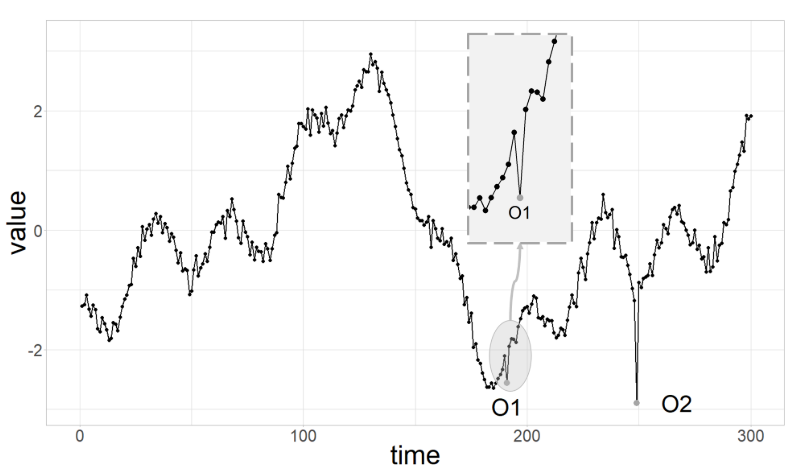
\includegraphics[width=10cm]{Cap2_LitReview/point_anomaly.png}
    \caption{\cite{Blázquez-García_Conde_Mori_Lozano_2021}}
    \label{fig:point_anomaly}
\end{figure}

\begin{figure}[H]
    \centering
    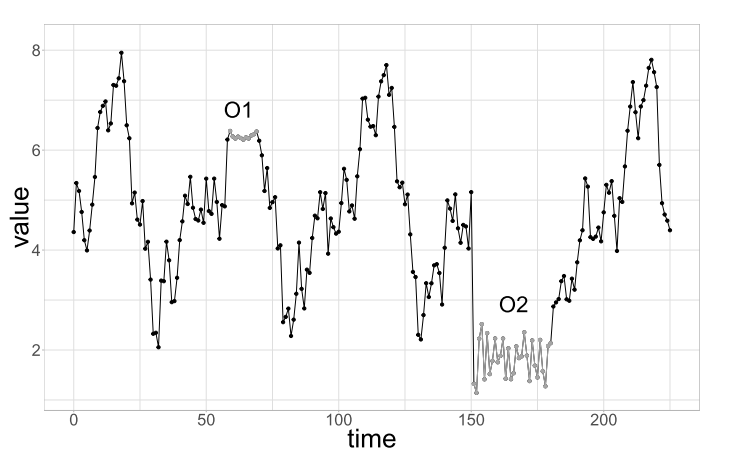
\includegraphics[width=10cm]{Cap2_LitReview/subseq_anomaly.png}
    \caption{\cite{Blázquez-García_Conde_Mori_Lozano_2021}}
    \label{fig:subsequence_anomaly}
\end{figure}

\begin{figure}[H]
    \centering
    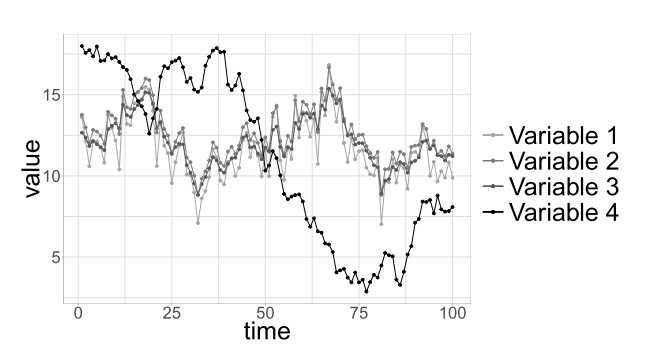
\includegraphics[width=10cm]{Cap2_LitReview/TS_anomaly.png}
    \caption{\cite{Blázquez-García_Conde_Mori_Lozano_2021}}
    \label{fig:Time_series_anomaly}
\end{figure}

\section{Time Series Anomaly Detection Models}

Since the 1960s, many models for anomaly detection have been proposed, ranging from statistical models to recent deep learning models. The common main idea behind all of those is to identify low probability, i.e. low density, regions, classifying points in those areas as anomalies \cite{Samariya_Thakkar_2021}. 

Statistical models, for example, use statistical tests, like the $\chi ^2$ test, to identify abnormal points. Clustering-based models use cluster analysis to label anomalies, using, for example, the distance from the centroid of normal points or the number of points in a cluster. Distance-based models use the distance between the current time window and its neighborhood to classify anomalies. Density-based approaches use the density of the data points to find anomalies \cite{Zamanzadeh_Darban_Webb_Pan_Aggarwal_Salehi_2024, Samariya_Thakkar_2021}. These methods described above are called traditional methods.

In recent years, with the increase of computing power, deep learning models have become increasingly prominent in anomaly detection. Unlike the traditional methods, the main advantage of deep learning models is that they are capable of identifying complex temporal and spatial correlations between variables, especially in larger multidimensional datasets, without the need for a labeled dataset \cite{Zamanzadeh_Darban_Webb_Pan_Aggarwal_Salehi_2024, Choi_Yi_Park_Yoon_2021}. \cite{Zamanzadeh_Darban_Webb_Pan_Aggarwal_Salehi_2024} divides deep learning models into 3 main categories: forecasting-based models, reconstruction-based models, and representation-based models.

Forecasting-based models try to predict a future subsequence of the time series using historical data. These models learn the patterns and trends within data to anticipate what is expected to occur. Recurrent Neural Networks (RNNs) and Long Short-Term Memory (LSTMs) are examples of this category. Anomalous values are detected if they deviate greatly from what the model predicts.

Reconstruction-based models attempt to recreate the input timeseries based on the values of past points or windows. These models use architectures like autoencoders (AE) and Generative Adversarial Networks (GANs). Anomalies are identified using the reconstruction error between the predicted series and the original series. The advantage of reconstruction-based models over forecasting ones is that they adapt better to rapid changes in a timeseries, which may cause it to become unpredictable. This happens because reconstruction models have access to the current timeseries data, which is not available in forecasting models \cite{Zamanzadeh_Darban_Webb_Pan_Aggarwal_Salehi_2024}. This better precision comes with a delay in the detection time of an anomaly, but, in general, these models are preferred over forecasting models.

Representation-based models focus on learning meaningful representations of the data that can be used in downstream tasks, like anomaly detection.  These models use advanced architectures like transformers and self-supervised learning to extract high-level features from the data. The learned representations are often used in conjunction with simpler models (e.g., clustering or density-based methods) to identify anomalies. The downside of these models is that they are computationally expensive to train, often needing a large amount of data.

An important point to highlight is that the majority of the models described above are unsupervised models. An unsupervised model is a model that can learn patterns from data without the need for a labeled dataset. This flexibility is desired because of the inherently unlabeled nature of historical data and the unpredictability of anomalies, which makes it harder to define an anomaly, especially if anomalies are rare. In this work, the focus will be on unsupervised reconstruction models.

Another important point to note is that, as will be detailed in Sections \ref{sec-track-quality-accel} and \ref{sec-methodology}, the model proposed in this thesis is not designed specifically for anomaly detection. Instead, its primary objective is to learn how to reconstruct track irregularities from acceleration data. Despite that, the main idea that motivates the model's development is closely related to anomaly detection. For this reason, a review of anomaly detection methods was included.

\section{Basics of Deep Learning Models}

Before diving deeper into anomaly detection models, the fundamental concepts of deep learning will be presented first. This preliminary discussion will provide the necessary context and theoretical basis for the subsequent exploration of anomaly detection methodologies.

\subsection{Neural Networks} \label{sec-Neural_networks}

Neural networks are the most basic structure in deep learning. It is inspired by the way the human brain works \cite{AGATONOVICKUSTRIN2000717,Alzubaidi_Zhang_Humaidi_Al-Dujaili_Duan_Al-Shamma_Santamaría_Fadhel_Al-Amidie_Farhan_2021}. These networks are composed of thousands, or even millions, of interconnected units called perceptrons, which mimic the behavior of biological neurons. In a neural network, these perceptrons are arranged into multiple layers, as shown in Figure \ref{fig:neural_network-a}. In this illustration, each circle represents a single perceptron. 

The neural network is divided into three main components: 
\begin{itemize}
    \item The input layer: this layers receives raw data that will be precessed;
    \item The hidden layers: positioned between the input and output layers, these intermediate layers perform feature extraction;
    \item The output layer: this layer provides predictions or classifications
\end{itemize}

Each perceptron in a neural network processes input data linearly using the dot product. Given, them, an input array $\mathbf{x}$, the perceptron computes the output by multiplying $\mathbf{x}$ with an array of weights $\mathbf{w}$ and adding a bias $b$, producing a scalar output $o$ \cite{Gurney_1997}:
\begin{equation}
    o = \sum_{i}w_i x_i + b
\end{equation}

The weights and biases are learned and iteratively updated during the training process such that they minimize the errors.

However, in its basic form, a perceptron can only solve linearly separable problems. To address this limitation, modern perceptrons include an additional element: the activation function. An activation function introduces non-linearity into the model, enabling it to solve complex, non-linear problems \cite{Roth_2016}.For reasons that will be explained later, it is common to choose differentiable activation functions. Common activation functions include the Rectified Linear Unit (ReLU) and the hyperbolic tangent (tanh). The general structure of a perceptron, including the activation function, is illustrated in Figure \ref{fig:neural_network-b}.

%\begin{figure}[H]
 %   \centering
  %  \includegraphics[width=0.5\linewidth]{Cap2_LitReview/model_basics/Colored_neural_network.png}
   % \caption{\cite{enwiki:1294206888}}
    %\label{fig:neural_network}
%\end{figure}

\begin{figure}[H]
    \centering
    \begin{subfigure}{0.45\textwidth}
        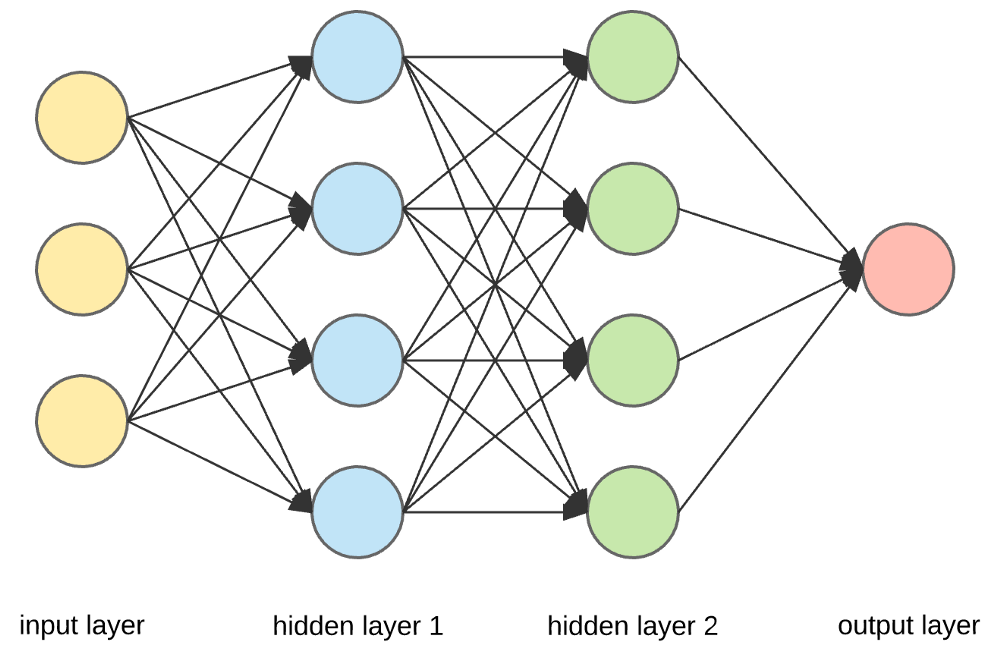
\includegraphics[width=7cm]{Cap2_LitReview/model_basics/Neural_networks/neural_network.png}
        \caption{\cite{P._2025}}
        \label{fig:neural_network-a}
    \end{subfigure}
    \hspace{0.2cm}
    \begin{subfigure}{0.45\textwidth}
        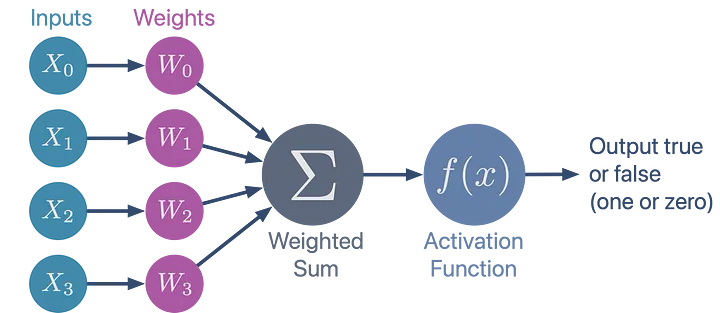
\includegraphics[width=8cm]{Cap2_LitReview/model_basics/Neural_networks/perceptron.png}
        \caption{\cite{Weaver_2024}}
        \label{fig:neural_network-b}
    \end{subfigure}
    \caption{Caption}
    \label{fig:neural_network}
\end{figure}

As mentioned earlier, the weights and biases of the perceptrons are adjusted and optimized during the training phase of a neural network. This optimization process involves a method called backpropagation, which is essential for minimizing the error in predictions. Backpropagation, discussed in detail in Section \ref{sec-backpropagation}, leverages the gradient descent algorithm to iteratively update the network's parameters, ensuring improved accuracy over successive training iterations.

\subsection{Backpropagation} \label{sec-backpropagation}

During the training phase of a neural network, its weights and biases are systematically optimized to minimize the error. This iterative process comprises two key subprocesses: a forward pass followed by a backward pass. In a forward pass, the inputs are passed through the network and the outputs are calculated. Then, given an expected output, an error is computed using a function called the loss function. The backward pass, then, uses this error to update the weights and biases of the neural network, making it better at making right predictions. This process continues until the error is small enough.

The process of propagating the error back through the network during the backward pass is referred to as backpropagation. It can be broken down into four primary steps \cite{cilimkovic2015neural}:

\begin{enumerate}
    \item Feed foward the inputs;
    \item Backpropagation to the output layer;
    \item Backpropagation to the hidden layers;
    \item Weights updates.
\end{enumerate}

The first step is just feeding forward the inputs $\mathbf{x}$ through the network and obtaining the outputs $\mathbf{o}$. Then, a loss is computed using the loss function $\mathbf{L}$. There are a variety of loss functions, an example being the Mean Squared Error (MSE):
\begin{equation}
    \mathbf{L} = \frac{1}{N} \sum_{i} \left(y_i-o_i\right)^2
\end{equation}
where $y_i$ is the desired output and $o_i$ is the network output. To backpropagate the error, the algorithm computes gradients of the loss function with respect to the parameters of the neural network. This is done using the chain rule twice \cite{Roth_2016}:
\begin{equation}
    \frac{\partial \mathbf{L}}{\partial w_{ij}} = \frac{\partial \mathbf{L}}{\partial o_j}
    \frac{\partial o_j}{\partial net_j}\frac{\partial net_j}{\partial w_{ij}}
\end{equation}
where $w_{ij}$ is the i-th weight of the j-th perceptron, $net_j$ is the result of the dot product before applying the activation function, i.e.,
\begin{equation}
    net_j = \sum_i w_{ij} x_j
\end{equation}
with $x_j$ being the input, and $o_j$ the perceptron output, i.e.,
\begin{equation}
    o_j = \varphi (net_j)    
\end{equation}
where $\varphi$ is the activation function of the perceptron. For this reason, it is necessary that the activation function is a differentiable function. 

To update the weights, the algorithm computes, then, the incremental $\Delta w_{ij}$ using:
\begin{equation}
    \Delta w_{ij} = -\eta \delta_j x_{ij}
\end{equation}
where $\eta$ is a small positive number known as the learning rate, $\delta_j = \frac{\partial \mathbf{L}}{\partial net_j}$ and $x_{ij}$ are the inputs of the j-th perceptron, and, thus, update the weights as:
\begin{equation}
    w_{ij} \xleftarrow{} w_{ij} + \Delta w_{ij}
\end{equation}
For a full demonstration of these formulas, check Appendix \ref{appendix-a}. 

Despite its effectiveness, the classical backpropagation algorithm has some problems associated with its convergence. For example, if the learning rate is too small, the convergence is very slow and can converge to a local minimum; on the other hand, if it is too large, the algorithm can diverge \cite{ruder2016overview}. Several modifications to the original algorithm have been proposed, like in \cite{QIAN1999145}, \cite{1370017282431050757} and \cite{kingma2017adammethodstochasticoptimization}, but the contents of these works are outside the scope of this thesis. 

\subsection{Convolutional Neural Networks} \label{section-CNN}
%Escrever sobre treinamento, dps backpropagation e adam, CNN, LSTM, transformers.
Convolutional neural networks (CNN) achieved great popularity in modern machine learning, gaining large popularity with the \cite{NIPS2012_c399862d} paper. In this work, the authors proposed a deep CNN that won the ImageNet LSVRC-2010 contest, outperforming second place by a large margin. 

A CNN, similarly to the neural network, was inspired by the biological neurons, but, different from the conventional neural network, where all the neurons are connected and interact with all neurons in adjacent layers, the CNN employs a sparse architecture, i.e., the neurons are connected only to a local region of the input. This sparsity reduces the amount of training parameters, which reduces the computational cost and speeds up the training process \cite{Alzubaidi_Zhang_Humaidi_Al-Dujaili_Duan_Al-Shamma_Santamaría_Fadhel_Al-Amidie_Farhan_2021, 9451544}. 

CNNs are widely used in computer vision to process and analyze 2D images and are used to solve a variety of image-related problems, like classification and object detection. While this section focuses on explaining CNN concepts with the assumption of a 2D input, it is important to note that the principles discussed are equally applicable to 1D inputs, like in a timeseries.

The basic block of a CNN is the convolution operation. A convolution can be defined as the dot product between an input $x$ of shape $(m,m,r)$, where $m$ is the height, which is the same as the width, and $r$ is the depth, also called the channel number, and $k$ convolutional filters, called kernels. A kernel is a grid of weights, with shape $(n,n, q)$, where $n < m$ and $q \leq r$, that convolves with the input, producing, each, an output of size $(m-n-1)$, called the feature maps \cite{Alzubaidi_Zhang_Humaidi_Al-Dujaili_Duan_Al-Shamma_Santamaría_Fadhel_Al-Amidie_Farhan_2021}. These kernels compute the pass value similarly to the 
\begin{equation}
    h^k = f\left(W^k * x + b_k\right)
\end{equation}

where $W^k$ is the vector of weights from the kernel, $f$ is an activation function, and $b^k$ is the bias. Figure \ref{fig:conv-example} shows an example of this operation between a 2D binary matrix and a $3\times3$ kernel. 

\begin{figure}[H]
    \centering
    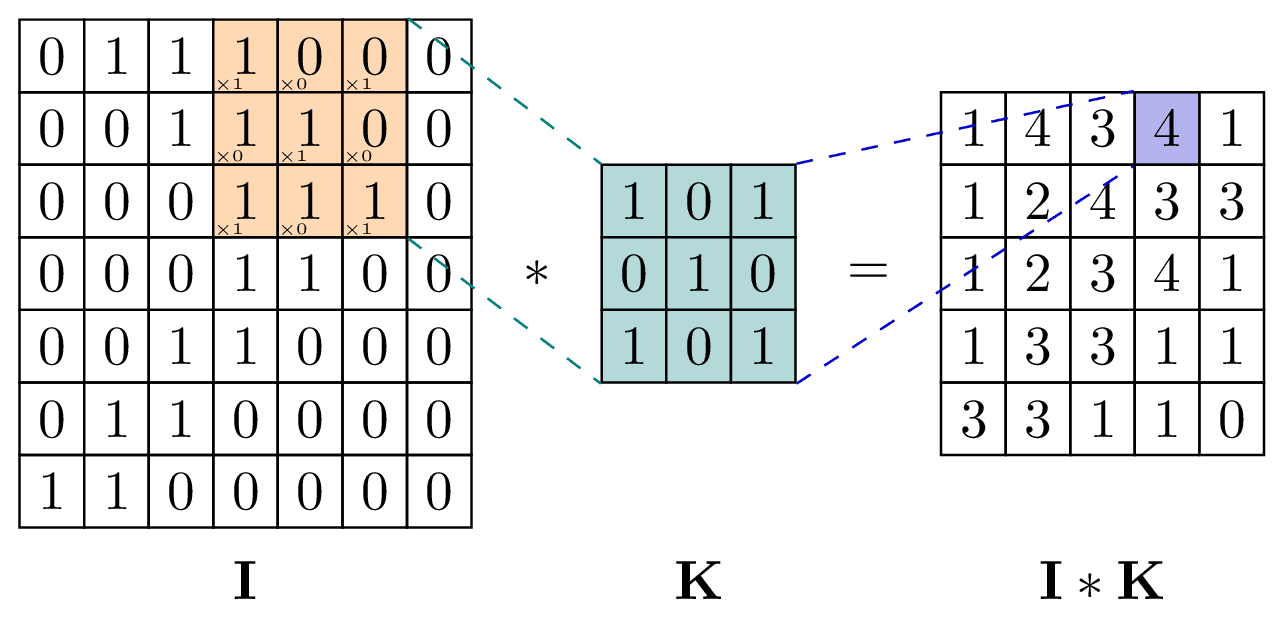
\includegraphics[width=9cm]{Cap2_LitReview/model_basics/Convolutional_NN/conv2d.png}
    \caption{\cite{Riebesell_2022}}
    \label{fig:conv-example}
\end{figure}

In addition to the convolution operation, there are two other important parameters in convolutional neural networks: the padding and the stride. Their main function is to control the output size of the convolution, helping to maintain the spatial characteristics of the input. 

The padding is the process of adding additional rows and columns around the border of the input matrix, typically filled with zeros, a process known as zero padding. Without the padding, a convolution with a kernel of size $n\times n$ reduces the output size by $n-1$ in each spatial dimension. This would cause a rapid decrease in the size of the features, that would force the use of small kernels \cite{Goodfellow_Bengio_Courville_2018}.

Stride, on the other hand, controls how the kernel moves across the input matrix, by skipping some of the elements from it. In a stride 1 convolution, the kernel shifts one unit at a time, covering all the positions. In a stride 2 convolution, the kernel would shift 2 elements each time, which causes the kernel to convolve with every other element. In general, a stride of size $s$ means that the kernel will only convolve every $s$ elements. This is done primarily to reduce computational cost, at the expense of extracting the features less finely \cite{Goodfellow_Bengio_Courville_2018}. 

Now with these two additional operations, the output size can be computed using the formula:
\begin{equation}
    O = \left\lfloor \frac{I + 2 \cdot p - k}{s} \right\rfloor + 1
    \label{eq:conv_output}
\end{equation}
where $O$ is the output size, $I$ is the input size, $p$ is the padding, $k$ is the kernel size, and $s$ is the stride.

Another important feature that is widely used in CNNs is the pooling layer. Pooling layers are used to further reduce the spatial dimension of the feature map by replacing the output value of the convolution operation with a local summary statistic, which helps the model to develop representations that are invariant to small translations \cite{Goodfellow_Bengio_Courville_2018}. 

One of the most widely used types is max pooling, which selects the maximum value within a local neighborhood, as shown in Figure \ref{fig:pooling-example}. Other common pooling methods include average pooling, which computes the mean of the values within the region, and weighted average pooling, where each value contributes proportionally based on predefined weights.

\begin{figure}[H]
    \centering
    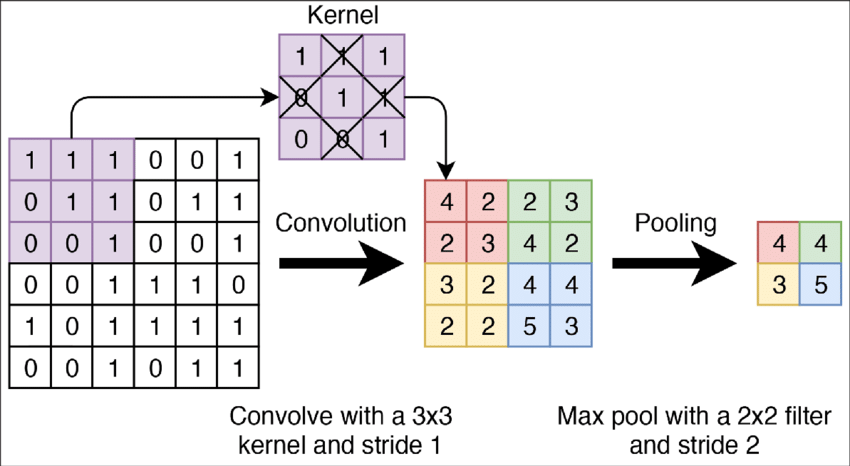
\includegraphics[width=9cm]{Cap2_LitReview/model_basics/Convolutional_NN/Schematic-representation-of-a-convolution-and-pooling-layer-in-a-CNN.png}
    \caption{\cite{Verschoof-van}}
    \label{fig:pooling-example}
\end{figure}

\section{Recurrent Neural Networks} \label{section-RNN}

Recurrent Neural Networks (RNNs) are a type of artificial neural network specifically designed to work with sequential data, such as time series, speech recognition, text generation, and language modeling \cite{schmidt2019recurrentneuralnetworksrnns,fang-wei,Alzubaidi_Zhang_Humaidi_Al-Dujaili_Duan_Al-Shamma_Santamaría_Fadhel_Al-Amidie_Farhan_2021}. The main difference between an RNN and the networks discussed in Sections \ref{sec-Neural_networks} and \ref{section-CNN} is how data is processed inside the RNN. In the MLP and the CNN networks, it is assumed that each input is independent from each other, which can be a valid assumption when dealing with images, but might be a severe limitation when dealing with sequential data, like weather data, where, for example, the current temperature depends on the last few measurements. 

RNNs deal with this kind of problem by introducing a cycle in their architecture  allows information to persist across time steps \cite{schmidt2019recurrentneuralnetworksrnns}, as shown in Figure \ref{fig:RNN-struct}. The key idea is to add a hidden-to-hidden weight matrix $\boldsymbol{W}_{hh}$ that carries information from the previous hidden state $\boldsymbol{H}_{t-1}$ in the computation of the current hidden state $\boldsymbol{H}_t$. 

The current hidden state can be computed using Equation \ref{eq-RNN-hidden}:
\begin{equation}
    \boldsymbol{H}_t = \phi(\boldsymbol{X}_t \boldsymbol{W}_{xh} + \boldsymbol{H}_{t-1} \boldsymbol{W}_{hh} + \boldsymbol{b}_h)
    \label{eq-RNN-hidden}
\end{equation}
where $\boldsymbol{X}_t$ is the input vector, $\boldsymbol{W}_{xh}$ is the input-to-hidden weight matrix, $\boldsymbol{b}_h$ is the bias, and $\phi$ is an activation function. 

An important observation is that it is not necessary to explicitly include all previous hidden states, from $\boldsymbol{H}_{0}$ up to $\boldsymbol{H}_{t-2}$, when computing $\boldsymbol{H}_t$. This is because, at each iteration, the RNN updates $\boldsymbol{H}_{t}$ by combining the input $\boldsymbol{X}_t$ with the previous hidden state $\boldsymbol{H}_{t-1}$, which is the result of the computation between $\boldsymbol{X}_{t-1}$ and $\boldsymbol{H}_{t-2}$, and so on recursively. This way, the network can keep information about the previous time steps when computing the next one.

\begin{figure}[H]
    \centering
    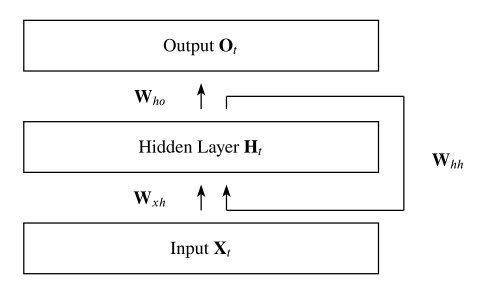
\includegraphics[width=9cm]{Cap2_LitReview/model_basics/RNN/rnn.png}
    \caption{Adapted from \cite{schmidt2019recurrentneuralnetworksrnns}}
    \label{fig:RNN-struct}
\end{figure}

The main problem in the original RNN architecture arises during the training phase, specifically when computing gradients for weight updates. As gradients are propagated backward through time, a series of repeated multiplications occurs. If these values are greater than 1, the gradients can grow exponentially, causing the network weights to change abruptly fast. Conversely, if the values are less than 1, the gradients decay exponentially, which causes the gradient to vanish \cite{kolen,pmlr-v9-glorot10a}. The vanishing gradient then causes the network to forget information from the initial time steps, which makes it difficult for RNNs to learn long-term dependencies in data.

This inherent problem motivated the introduction of more complex architectures, such as the LSTM networks. These networks will be explained in more detail in \ref{sec-LSTM}, but they mitigate the vanishing gradient problem, which caused the original RNNs to be barely used in today's research \cite{fang-wei,GAO2019279}.

\section{LSTM} \label{sec-LSTM}

Long Short-Term Memory (LSTM) units were introduced by Hochreiter and Schmidhuber in 1997 \cite{Hochreiter} and were specifically designed to deal with the vanishing gradient problem. Differently from vanilla RNNs, which struggle to retain information over long sequences, LSTM cells are specifically designed to capture long-term dependencies by preserving information across many time steps \cite{ALSELWI2024102068,schmidt2019recurrentneuralnetworksrnns}.

The core idea behind the LSTM architecture lies in its gating mechanism, which regulates the flow of information through the cell. This mechanism is composed of three gates: the forget gate, the input gate, and the output gate, shown in Figure \ref{fig:LSTM-struct}. Each gate uses a sigmoid activation function, producing values between 0 and 1 to determine how much information should pass through \cite{schmidt2019recurrentneuralnetworksrnns}.

\begin{itemize}
    \item The forget gate decides which parts of the previous cell state should be discarded, allowing the network to “forget” irrelevant or outdated information. 
    \item The input gate determines which portions of the new input information should be added to the cell state.
    \item The output gate controls which parts of the internal cell state are exposed as the output hidden state at the current time step.
\end{itemize}

The forget and input gates are responsible for updating the cell state, which acts as an internal memory, carrying forward important information throughout the sequence. The output gate, meanwhile, regulates how much of the updated cell state should influence the hidden state output. Through this mechanism, LSTMs are able to maintain and regulate long-term information flow \cite{ALSELWI2024102068}.

\begin{figure}[H]
    \centering
    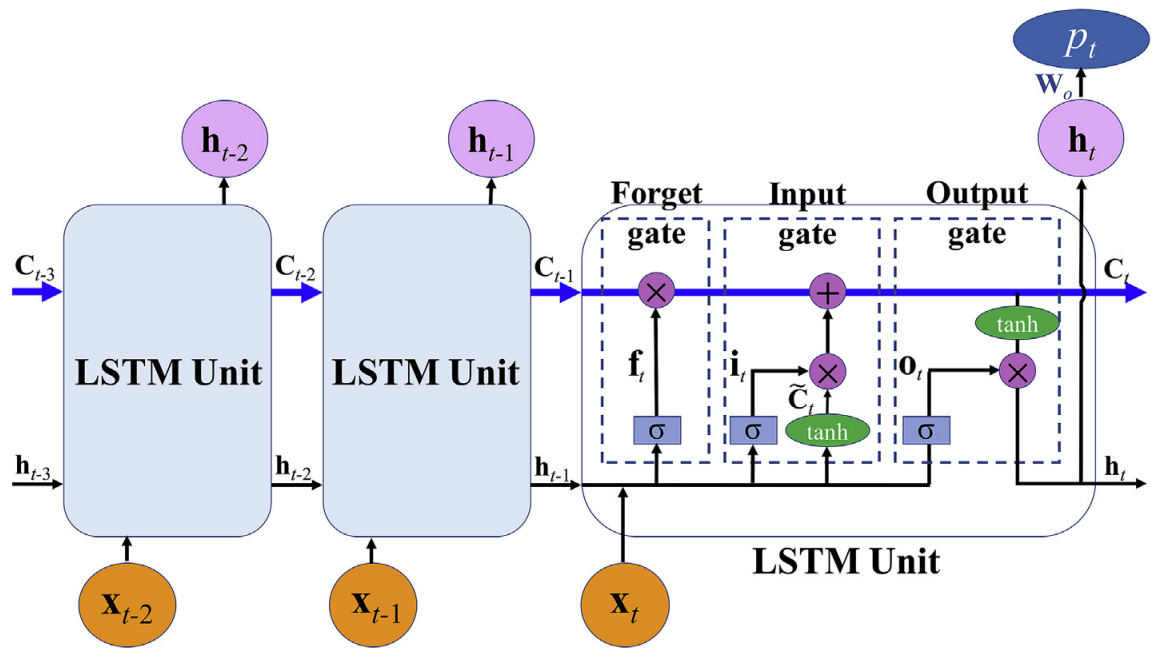
\includegraphics[width=9cm]{Cap2_LitReview/model_basics/LSTM/LSTM_Arch.png}
    \caption{Adapted from \cite{WEI2021453}}
    \label{fig:LSTM-struct}
\end{figure}

Using the same notation from Section \ref{section-RNN} one can compute:
\begin{equation}
    \boldsymbol{O}_t = \sigma\left(\boldsymbol{X}_t \boldsymbol{W}_{xo} + \boldsymbol{H}_{t-1}\boldsymbol{W}_{ho} + \boldsymbol{b}_o\right)
    \label{eq-LSTM-Ot}
\end{equation}
\begin{equation}
    \boldsymbol{I}_t = \sigma\left(\boldsymbol{X}_t \boldsymbol{W}_{xi} + \boldsymbol{H}_{t-1}\boldsymbol{W}_{hi} + \boldsymbol{b}_i\right)
    \label{eq-LSTM-It}
\end{equation}
\begin{equation}
    \boldsymbol{F}_t = \sigma\left(\boldsymbol{X}_t \boldsymbol{W}_{xf} + \boldsymbol{H}_{t-1}\boldsymbol{W}_{hf} + \boldsymbol{b}_f\right)
    \label{eq-LSTM-Ft}
\end{equation}
where $\boldsymbol{O}_t$, $\boldsymbol{I}_t$, and $\boldsymbol{F}_t$ are the inputs for the output gate, the input gate, and the forget gate, respectively. After this computation, the LSTM unit computes the candidate memory cell $\boldsymbol{\tilde{C}}_t$, which represents the candidate information that could be added to the cell state, as:
\begin{equation}
    \boldsymbol{\tilde{C}}_t = \tanh \left(\boldsymbol{X}_t \boldsymbol{W}_{xc} + \boldsymbol{H}_{t-1}\boldsymbol{W}_{hc} + \boldsymbol{b}_c\right)
    \label{eq-CNN-Candidate}
\end{equation}

After that, the LSTM introduces the previous memory content $\boldsymbol{C}_{t-1}$, which, together with the other gates, controls how much of the old memory information will be retained in the new memory state $\boldsymbol{C}_{t}$, which can be computed using: 
\begin{equation}
    \boldsymbol{C}_t = \boldsymbol{F}_t \otimes \boldsymbol{C}_{t-1} + \boldsymbol{I}_t \otimes \boldsymbol{\tilde{C}}_t
\end{equation}
where $\otimes$ denotes the element-wise multiplication. Finally, the LSTM unit computes the hidden state $\boldsymbol{H}_t$ as:
\begin{equation}
    \boldsymbol{H}_t = \boldsymbol{O}_t \otimes \tanh (\boldsymbol{C}_t)
\end{equation}

It is important to notice the hidden state $\boldsymbol{H}_t$ is used as the output of the LSTM cell and, together with the memory state $\boldsymbol{C}_t$, is used in the computation of the next time step.

\section{Attention}

Attention is an important concept in deep learning that was first introduced by \cite{bahdanau2016neuralmachinetranslationjointly} in a machine translation problem and gained widespread popularity with the famous paper "Attention Is All You Need" proposed by \cite{vaswani2023attentionneed}, where the authors proposed the transformer architecture. Inspired by the human attention of selectively focusing on relevant information, attention mechanisms enable neural networks to assign different weights to different parts of the input, allowing the model to concentrate on the most important elements of the data. This selective focus not only improves the model's interpretability but also makes it possible to handle large amounts of information more efficiently, reducing computational overhead \cite{NIU202148}.

The attention mechanism works by taking a vector of features $\boldsymbol{F}$, which are obtained after the input data $\boldsymbol{X}$ is passed through a feature extraction model to extract the feature vectors $\boldsymbol{f}_1$, to $\boldsymbol{f}_n$. This feature extractor can vary depending on the task and, in the case of time series analysis, for example, it could be an encoder composed of CNNs, MLPs, or LSTMs, that produces the latent representations $\boldsymbol{f}_1$ to $\boldsymbol{f}_n$ \cite{Brauwers_2023}.

From the feature vectors $\boldsymbol{F}$ the model then extracts the key and value vectors $\boldsymbol{K}$ and $\boldsymbol{V}$, respectively. These vectors are usually obtained through a linear transformation of $\boldsymbol{F}$ using the weight matrix $\boldsymbol{W}_K$ and $\boldsymbol{W}_V$.

After that, the model introduces a query vector $\boldsymbol{Q}$, which is a task-specific vector that guides the attention mechanism to focus on the most important vectors \cite{Brauwers_2023,NIU202148}. From the query and key vectors, the model then computes the energy score $\boldsymbol{e}$ using a score function $f$:
\begin{equation}
    \boldsymbol{e} = f\left(\boldsymbol{Q},\boldsymbol{K}\right)
\end{equation}
where $f$ can be a variety of functions, such as the scaled dot product \cite{vaswani2023attentionneed}:
\begin{equation}
    f\left(\boldsymbol{Q},\boldsymbol{K}\right) = \frac{\boldsymbol{Q}^T \boldsymbol{K}}{\sqrt{d_k}}
\end{equation}

The energy scores $\boldsymbol{e}$ are then mapped to the attention weights $\boldsymbol{\alpha}$ using an attention distribution function $\mathrm{g}$, usually the softmax function \cite{NIU202148}:
\begin{equation}
    \boldsymbol{\alpha} = \mathrm{g}(\boldsymbol{e})
\end{equation}

Using the attention weights $\boldsymbol{\alpha}$ and the value vector $\boldsymbol{V}$, the model computes the context vector $\boldsymbol{c}$ using:
\begin{equation}
    \boldsymbol{c} = \sum_{l=1}^{n} \alpha_l \boldsymbol{V}_l  
\end{equation}
where $\alpha_l \in \mathrm{R}^1$ is the weight of the l-th vector. Figure \ref{fig:Attention-struct} shows the architecture of the attention model.

\begin{figure}[H]
    \centering
    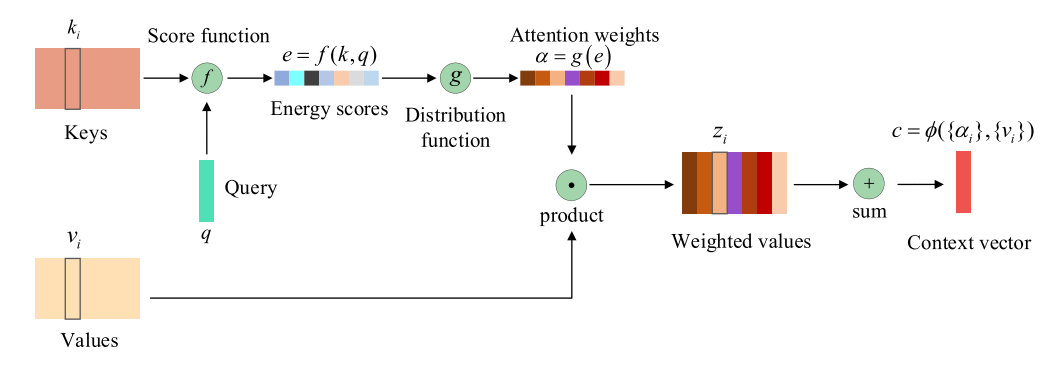
\includegraphics[width=12cm]{Cap2_LitReview/model_basics/Attention/attention-struct.png}
    \caption{\cite{NIU202148}}
    \label{fig:Attention-struct}
\end{figure}

\section{Transformers}



\section{Reconstruction-Based Models}

Reconstruction-based models are a class of machine learning models that are designed to learn the intrinsic correlations in data by trying to reconstruct the original input signal. Differently from forecasting-based approaches, which attempt to predict future values, reconstruction-based models focus on accurately recreating the current input. This approach makes them great for anomaly detection, often outperforming forecasting-based models because they have access to the current time series data, which helps them to be more stable to rapidly changing time series. However, this advantage comes with a trade-off because they introduce a delay in the detection of anomalies as they rely on reconstruction error analysis. \cite{Zamanzadeh_Darban_Webb_Pan_Aggarwal_Salehi_2024}. 

The main idea behind these networks is to train them to accurately reconstruct normal data, which is presumed to be the majority of the available data. This is usually done by minimizing a reconstruction loss, such as the Mean Squared Error (MSE), during the training phase. 

During the test phase, the model encounters anomalous data, which it has not been trained to reconstruct, causing the reconstruction error to increase greatly compared to the error of normal data, as the model fails to reconstruct abnormal patterns. This way, an anomaly can be identified by thresholding the reconstruction error. Inputs with low reconstruction error will be classified as normal, and inputs with reconstruction error greater than the threshold will be classified as anomalous.

There are a variety os reconstructions-based models, in Sections \ref{subsec-AE} and 
TODO: terminar de escrever sobre os modelos, escrever sobre defeitos, escrever sobre remocao do efeito de velocidade

\section{Railway Components}

The railway track consists of different interdependent components that are divided into two categories: the superstructure and the substructure. The former comprises the rails, fastenings, and sleepers, while the latter consists of the ballast, sub-ballast, and subgrade \cite{kaewunruen12008dynamic}, as shown in Figure ???. These two structures are separated by the sleeper-ballast interface and are essential for ensuring a safe and cost-effective transportation system capable of guiding vehicles and transmitting loads to the subgrade \cite{attoh2017big}.

INSERIR FIGURA AQUI


%TODO: Adicionar as seguintes seções futuramente: railway geometry and dynamics, railway defects, railway data collection and maintenance

\section{Railway Track Irregularities} \label{sec-track-defects}

Railway track defects 

\section{Assessing Railway Track Condition} \label{sec-assessing-railway-track}

Maintaining railway tracks in good condition is crucial to ensure safe and comfortable operations of trains \cite{Tsunashima-2019,GHIASI2025109516}. This maintenance is achieved through continuous monitoring of track conditions and the detection of irregularities. There are now two main methods to assess track quality: using track geometry cars (TGC) to directly measure the physical geometry of the track, and monitoring the dynamic response of the train using instrumented railway vehicles (IRV) equipped with onboard sensors capable of measuring the dynamics of the system \cite{PIRES2024107191}.

TGCs are equipped with sophisticated systems that directly measure the geometry of the track, that can be later compared to regulatory standards limits to identify parts of the track that need maintenance. However, this method has several drawbacks \cite{PIRES2024107191,GHIASI2025109516,Hironori_ONO202322-00239}:
\begin{itemize}
    \item Operational disruption: the operation of the railway track needs to be disrupted during the TGC inspection, which can halt operations for several hours depending on the length of the track being measured;
    \item Operational high cost: the sophisticated equipment and logistics make TGC operation costly, which limits their frequent use;
    \item Low inspection frequency: normally, the TGC measures the condition of the track monthly, due to its high cost, which is a problem if a fault appears between inspections.
\end{itemize}

To overcome the limitations in TCGs, an alternative approach was developed using IRVs equipped with sensors that measure the vehicle's dynamic response due to track excitations. The underlying principle behind IRVs is that the vehicle's vibrations are deeply correlated to track excitations \cite{PIRES2024107191,Tsunashima-2019}, and an irregularity in the track will cause an anomalous dynamic response from the vehicle, which can be identified in the sensors' readings. 

Using IRVs instead of the TCGs has several advantages, such as \cite{PIRES2024107191,GHIASI2025109516,Hironori_ONO202322-00239}:
\begin{itemize}
    \item No disruptions: the operation is not halted during the measurements, since data can be collected during normal train services, which reduces the costs with logistics;
    \item Real time data collection: data is collected in real time, which speeds up possible defect detections;
    \item High frequency of inspections: Since the measurements are taken directly from in-service trains, IRVs enable near-continuous monitoring of track conditions, greatly increasing the inspection frequency.
\end{itemize}

Despite that, it is important to highlight that data collection using IRVs also comes with some drawbacks, such as \cite{PIRES2024107191,GHIASI2025109516}:
\begin{itemize}
    \item High amount of data: the amount of data collected during IRV operation can be huge. This data needs to be carefully processed to obtain good quality data;
    \item Domain problem: different operations conditions, such as the wagon mass or velocity, can affect the dynamic response of the vehicle, so data collected from a one part of the track can be inherently different from another part;
    \item Correlation: since the measurements are done indirectly, they need to be correlated to the track condition, which can be a complex task that often needs the use of deep learning models;
    \item Data imbalance: since fault measurements are much more uncommon than normal measurements, the machine learning model needs to deal with class imbalance.
\end{itemize}

\section{Velocity Effect on Train Dynamics} \label{sec-vel-effect-measurement}

Train vibration measurements are strongly correlated to the velocity at which these measurements took place. As the wagon moves along the track, changes in velocity can alter the vibration responses measured by onboard sensors. At lower speeds, the dynamic response of the train to the track excitations tends to produce lower acceleration values than expected, while, for the same part of the track, higher velocities generate higher values of acceleration measured \cite{Hironori_ONO202322-00239}. Figure \ref{fig:vel_effect_ono} shows this difference in measurement found by \cite{Hironori_ONO202322-00239}. 

In Figure \ref{fig:vel_effect_ono-a}, the authors highlight two distinct velocity profiles labeled A and B, where the speed ratio between B and A is approximately 3. This difference in speed causes a significant change in the measured signal, as shown in Figure \ref{fig:vel_effect_ono-b}, where the velocity profile B generated bigger acceleration measures than A despite them traversing the same part of the track. 

To address this velocity-induced distortion, the authors propose two different correction methods. The first method involves using the Mahalanobis distance to distinguish outliers from normal data. After that, the authors fitted a linear regression to normal data to predict the expected acceleration given the speed. The measurements are then normalized by dividing them by their predicted values. 

In the second method, the authors employed a Gaussian process regression to model the behavior of acceleration and speed, obtaining a regression that mapped the velocity to the expected acceleration. Similarly, they normalized the measurements by their respective predictions. 

Both methods proved to be effective in mitigating the velocity effect, which reduced the number of false positives in anomaly detection, as shown in Figure \ref{fig:vel_correction_ono}.

\begin{figure}[H]
    \centering
    \begin{subfigure}{0.45\textwidth}
        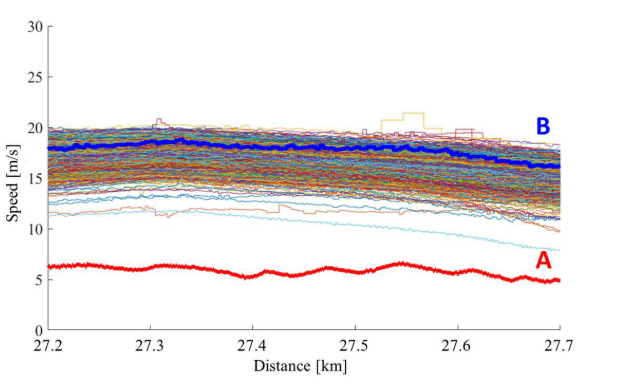
\includegraphics[width=8cm]{Cap2_LitReview/Vel_effect/vel_profiles.png}
        \caption{\cite{Hironori_ONO202322-00239}}
        \label{fig:vel_effect_ono-a}
    \end{subfigure}
    \hspace{0.3cm}
    \begin{subfigure}{0.45\textwidth}
        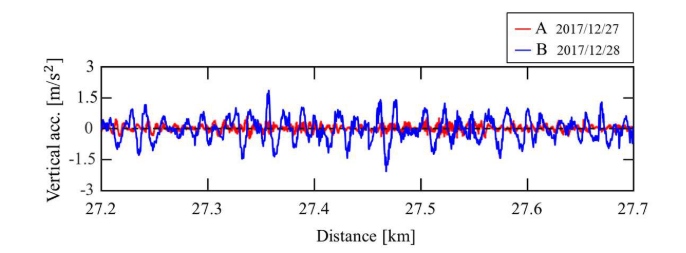
\includegraphics[width=8cm]{Cap2_LitReview/Vel_effect/accel_measurements.png}
        \caption{\cite{Hironori_ONO202322-00239}}
        \label{fig:vel_effect_ono-b}
    \end{subfigure}
    \caption{Caption}
    \label{fig:vel_effect_ono}
\end{figure}

\begin{figure}[H]
    \centering
    \begin{subfigure}{0.45\textwidth}
        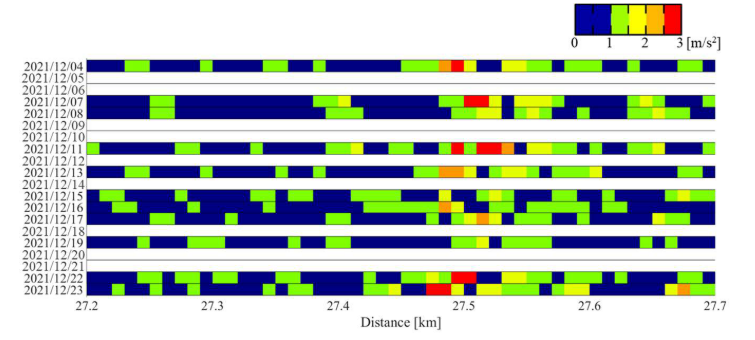
\includegraphics[width=8cm]{Cap2_LitReview/Vel_effect/before_correction.png}
        \caption{\cite{Hironori_ONO202322-00239}}
        \label{fig:vel_correction_ono-a}
    \end{subfigure}
    \hspace{0.3cm}
    \begin{subfigure}{0.45\textwidth}
        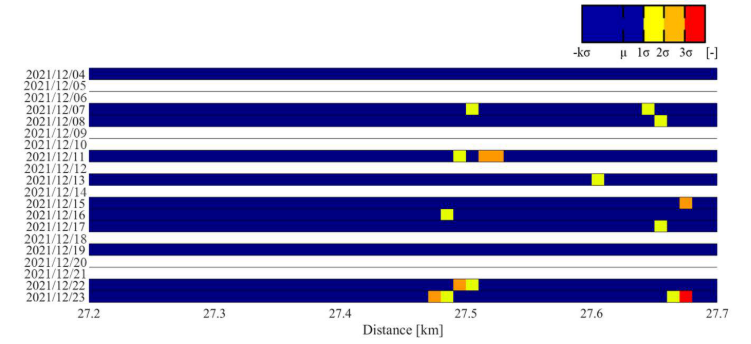
\includegraphics[width=8cm]{Cap2_LitReview/Vel_effect/after_correction.png}
        \caption{\cite{Hironori_ONO202322-00239}}
        \label{fig:vel_correction_ono-b}
    \end{subfigure}
    \caption{Caption}
    \label{fig:vel_correction_ono}
\end{figure}

Another example demonstrating the impact of the velocity on measured acceleration is presented in \cite{Balouchi02092021}. In this work, the authors utilized the VAMPIRE vehicle dynamics simulation software to model a vehicle operating in a measured track geometry at a variety of speeds. The simulated results were then compared to the actual car body vibration measurements recorded over the same section of the track. The results are shown in Figure \ref{fig:vel_effect_balouchi}, where the continuous colored lines are the simulation results, blue circles represent the maximum acceleration found in the simulation, and the dashed lines are the car body measurements. 

The authors fitted two models to the maximum simulated accelerations: a linear regression, the green line in Figure \ref{fig:vel_effect_balouchi} and an exponential model, the purple curve in Figure \ref{fig:vel_effect_balouchi}, to the maximum simulation acceleration, selecting the exponential model as it has a bigger $R^2$ value. They then argue that at lower speeds, the acceleration response does not yield a good level of confidence to differentiate if the quality of the track is good or bad, and so a normalization similar to \cite{Hironori_ONO202322-00239} is necessary.

\begin{figure}[H]
    \centering
    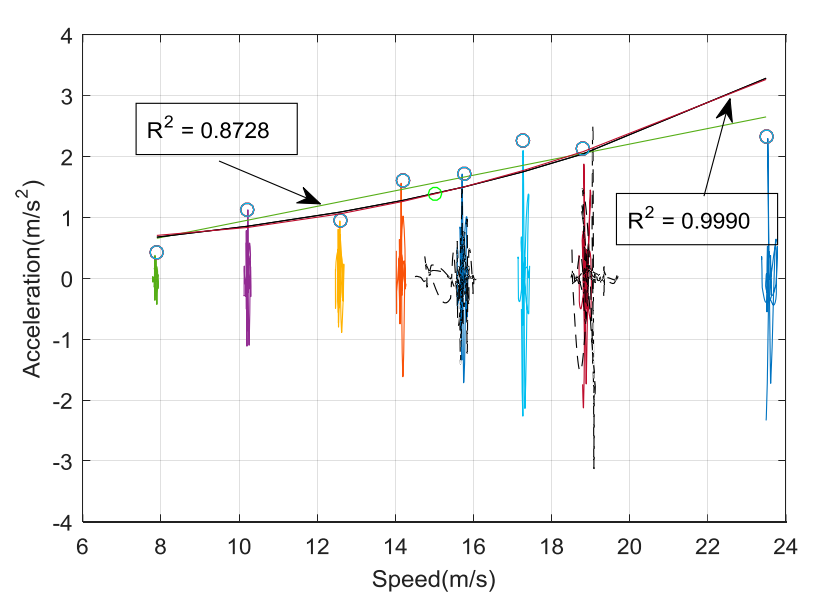
\includegraphics[width=12cm]{Cap2_LitReview/Vel_effect/results_bia.png}
    \caption{\cite{Balouchi02092021}}
    \label{fig:vel_effect_balouchi}
\end{figure}

\section{Assessing Track Quality from Acceleration Data} \label{sec-track-quality-accel}

As stated in Section \ref{sec-assessing-railway-track}, continuous measurements of track irregularities are an important factor in ensuring safety and comfort during railway operations. Traditionally, TGCs were used to assess track irregularities by directly measuring the track geometry. However, due to their high cost, constant inspection of the railway is not possible. 

An alternative to this approach is to use an IRV equipped with sensors that can measure the dynamic response of the vehicle due to track excitations. Normally, in this setup, accelerometers are mounted on various one or more components of the train, such as the axlebox, the bogie, or the car body, depending on the objective of the measurement and the maintenance costs of the sensors \cite{vibration7040049,Sansiñena26032025}. 

In \cite{Sansiñena26032025} authors presented a review of research papers that proposed methods for estimating track irregularities using acceleration data. They divided the methods into three main categories:
\begin{itemize}
    \item Model-driven methods;
    \item Data-driven methods;
    \item Hybrid methods.
\end{itemize}

In model-driven methods, a mathematical representation of the dynamic system is developed and validated on real data. Once the model accurately represents the system dynamics, the problem is inverted to estimate track irregularities from the measured acceleration data. The main advantage in model-driven methods is that they don't require a large amount of data to be designed, as they're based on expert knowledge. 

For instance, in \cite{DEROSA2019606} the authors used a 3D multibody model that was previously validated to measure the yaw and roll motions of the vehicle. Based on simulation data, they applied three reconstruction techniques, the Kalman filter, the Unknown Input Observer (UIO) and the Frequency Response Function (FRF), to reconstruct the lateral irregularities and the cross alignment. The performance of these methods was compared using two evaluation metrics, but the detailed results are out of the scope of this thesis. They then tested the FRF method on real measured data, which included lateral and vertical accelerations recorded at the axle-boxes, bogies, and car body, obtaining the reconstruction shown in Figure \ref{fig:DeRosa_Results}. The authors argue that although some similarity between the reconstructed and the original irregularities can be seen, the method did not produce satisfactory results. They justify that this deviation is caused by non-linear effects they didn't consider, but these deviations can occur because of the lack of robustness of the method to real-world noise in data, which is a common problem when dealing with simpler reconstruction methods.

\begin{figure}[H]
    \centering
    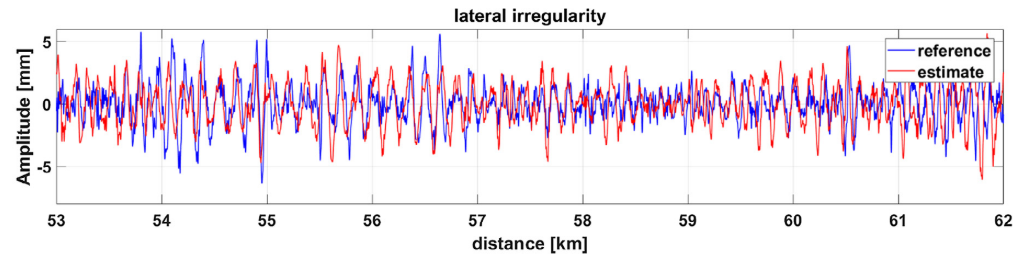
\includegraphics[width=12cm]{Cap2_LitReview/Track_Quality_Accel/DeRosa_Result_Real.png}
    \caption{\cite{DEROSA2019606}}
    \label{fig:DeRosa_Results}
\end{figure}

Data-driven methods, on the other hand, do not consider a mathematical model of the system, relying only on data processing to reconstruct or identify the irregularities. These methods typically utilize traditional machine learning algorithms or, more recently, deep learning architectures. Such approaches are generally more robust when dealing with real-world data, as they can learn from noisy and complex signals. This robustness, however, comes with a price, as they need a larger amount of data to be trained, especially in the case of deep learning \cite{Sansiñena26032025}. 

In \cite{vibration7040049} the authors propose a method of estimating railway track irregularities from car body vibration data. They first created a multibody simulation in SIMPACK. After that, they generated 12 different track irregularities, ranging from a good condition to a degraded condition, using FRA PSD formula and converted the generated profiles into 10 meters long track irregularity sections using the 10 m-chord versine method. This transformation is shown in Figure \ref{fig:Tsunashina_data_process}.

Using these irregularity profiles, they ran simulations over a 1000 meters track at speeds in the range of 40 to 80 km/h, varying the velocity in a 10 km/h interval. For each combination of track profile and speed, they collected the vertical and lateral acceleration as well as the roll rate of the carbody. Similarly to the irregularity profiles, a downsample was also applied to the data taking the maximum vibration measured in the 10 meters section, as shown in Figure \ref{fig:Tsunashina_data_process}. From this process, they obtained a dataset that correlates the maximum vibration of the carbody to the track irregularities for varying speeds and then applied a Gaussian Process Regressor (GPR) that was able to predict the irregularity from the vibration for a certain vehicle speed, as illustrated in Figure \ref{fig:Tsunashina_GPR}. 


\begin{figure}[H]
    \centering
    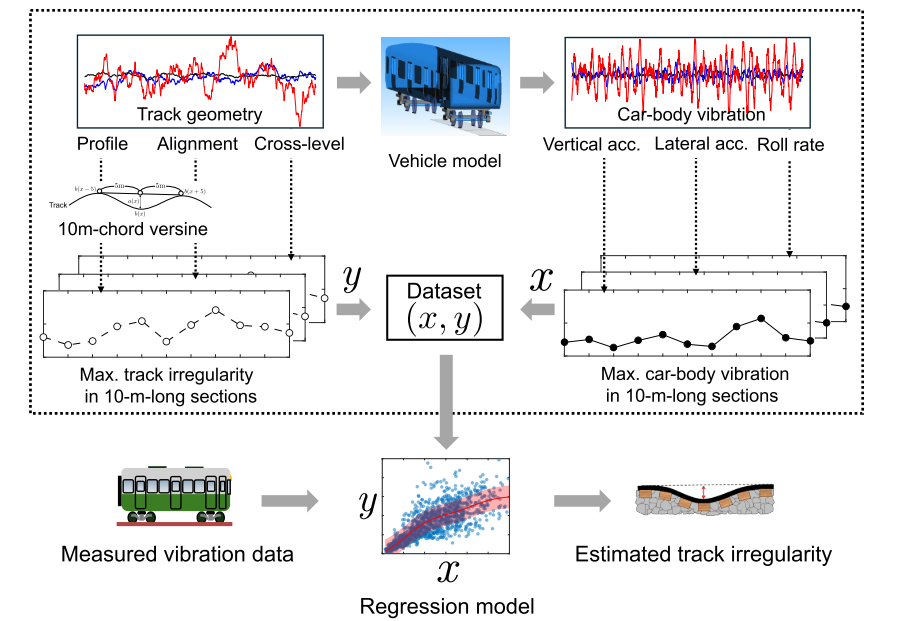
\includegraphics[width=12cm]{Cap2_LitReview/Track_Quality_Accel/Tsunashina (2024)/data-process.png}
    \caption{\cite{vibration7040049}}
    \label{fig:Tsunashina_data_process}
\end{figure}

\begin{figure}[H]
    \centering
    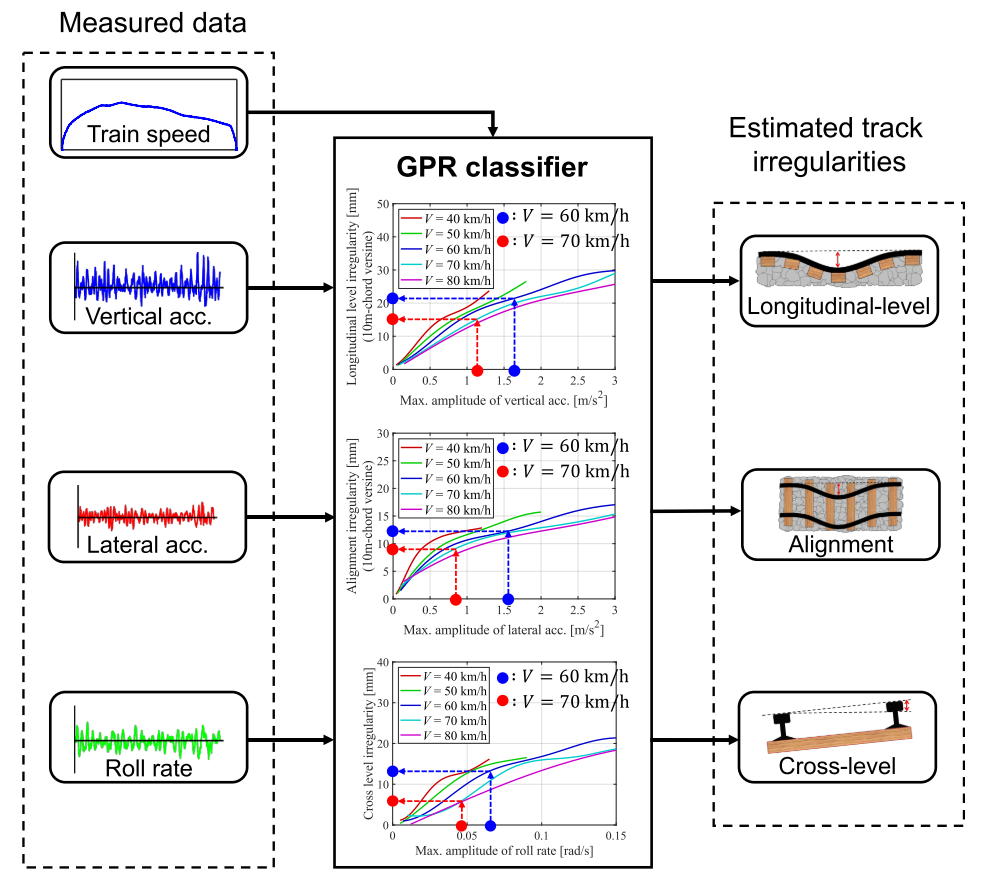
\includegraphics[width=12cm]{Cap2_LitReview/Track_Quality_Accel/Tsunashina (2024)/gpr.png}
    \caption{\cite{vibration7040049}}
    \label{fig:Tsunashina_GPR}
\end{figure}

The authors then tested their model utilizing real data measured using an onboard sensing device equipped with a triaxial accelerometer, a rate gyro, and a GNSS receiver. To ensure consistency, they applied the same downsample procedure to the real data and averaged the speed in the 10 m section to be used as an input for the regression model. The regression result for one part of the track is shown in Figure \ref{fig:Tsunashina_Results} and is presented with a 1$\sigma$ confidence interval. 

Tsunashima and Yagura argue that for the majority of the sections, the GPR predicts the correct value within the 1$\sigma$ confidence interval. However, for some of the sections, the predicted value significantly deviated from the actual measurement. They argue that there is a factor other than the track irregularity that influences the dynamics of the system and superimposes on the carbody's vibration. This difference might also occur because of the low complexity model used that might not have been able to learn the correlations between the variables very well. 

\begin{figure}[H]
    \centering
    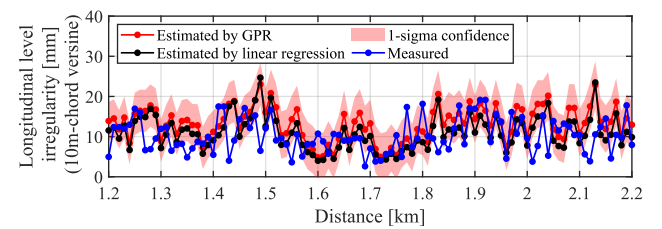
\includegraphics[width=12cm]{Cap2_LitReview/Track_Quality_Accel/Tsunashina (2024)/Results.png}
    \caption{\cite{vibration7040049}}
    \label{fig:Tsunashina_Results}
\end{figure}

In \cite{DeRosa2021}, the authors try to develop a threshold to detect not safe railway track irregularities. In the paper, the authors propose a machine learning-based classification model that divides the data into two classes based on the standard deviation of the lateral and roll bogie frame accelerations. Class 1 corresponds to normal conditions, i.e., track irregularities below a defined threshold that do not require maintenance, while Class 2 corresponds to sections with irregularities exceeding that threshold, thus requiring maintenance intervention. 

The authors use a dataset composed of real measurements collected onboard the high-speed TGC, operating at 300 km/h, that was also equipped with accelerometers located on the carbody, the bogie frames and the wheelsets, and a set of simulated data generated using a validated multibody dynamics model. From real data, the athor applies a pass-band filter in the range of 3 to 27 Hz and then computed the standard deviation of the signals over 100-meter-long track length. The simulation data was obtained considering a straight track, with a vehicle with speed of 300 km/h and for three different cases of track irregularities: considering only the lateral irregularity, considering only the cross level irregularity, and considering both at the same time. The authors didn't consider vertical irregularities in their simulation. For each case, they ran the simulation 10 times. The standard deviation was computed similarly to the real data. Figure \ref{fig:DeRosa-dataset} shows the whole dataset, where the red lines shown the standard defined limits for the standard deviation.

Using this dataset, the authors then fitted the data three classifiers: a decision tree, a linear Support vector Machine (SVM) and a Gaussian SVM. Results are shown in Table \ref{Table:DeRosa-2021-Results}. The authors state that 

\begin{figure}[H]
    \centering
    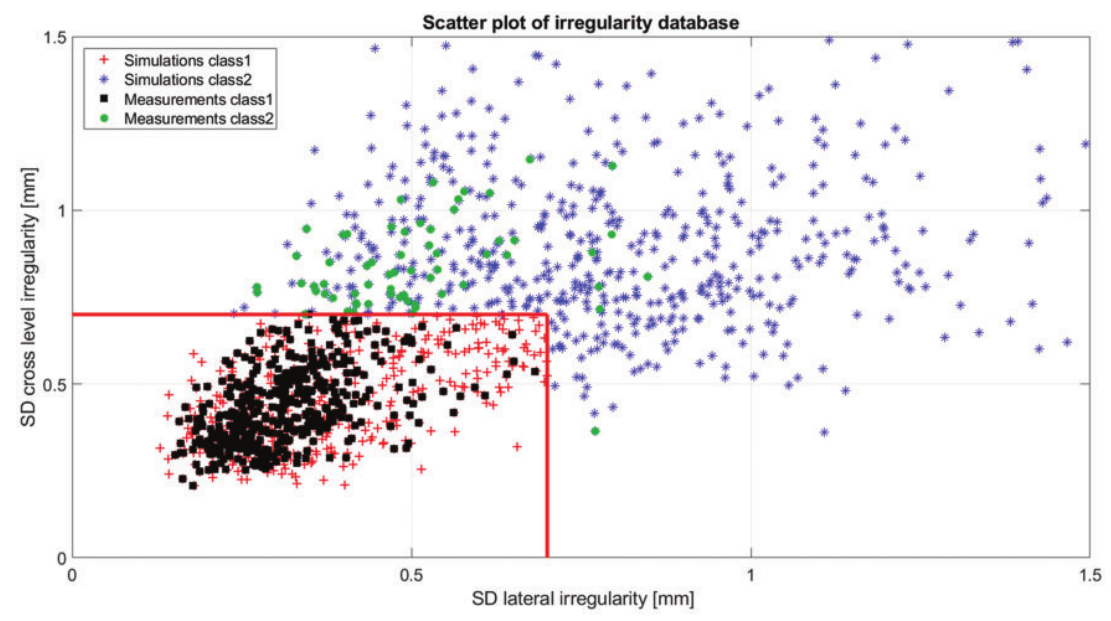
\includegraphics[width=12cm]{Cap2_LitReview/Track_Quality_Accel/DeRosa (2021)/dataset.png}
    \caption{\cite{DeRosa2021}}
    \label{fig:DeRosa-dataset}
\end{figure}

\begin{table}[ht]
\centering
\begin{tabular}{l c c c c c}
\hline
 & Accuracy (\%) & Precision (\%) & Recall (\%) & $F_1$ score (\%) & Kappa \\
\hline
Decision tree & 87.6 & 49.6 & 92.1 & 64.4 & 0.58 \\
Linear SVM & 92.9 & 70.3 & 71.4 & 70.9 & 0.67 \\
Gaussian SVM & 92.9 & 68.1 & 77.8 & 72.6 & 0.69 \\
\hline
\end{tabular}
\vspace{0.5em}
\small SVM: support vector machine.
\caption{Summary of classifier performances in the testing phase.}
\label{Table:DeRosa-2021-Results}
\end{table}


% \begin{figure}[H]
%     \centering
%     \begin{subfigure}{0.8\textwidth}
%         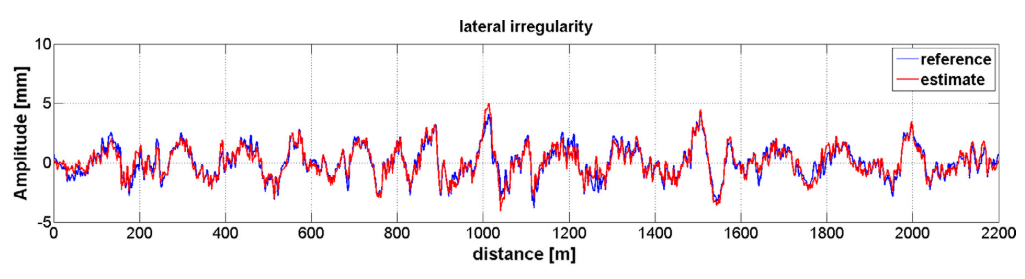
\includegraphics[width=8cm]{Cap2_LitReview/Track_Quality_Accel/DeRosa_Results_Freq.png}
%         \caption{Adapted from \cite{DEROSA2019606}}
%         \label{fig:deRosa_a}
%     \end{subfigure}
%     \\
%     \begin{subfigure}{0.8\textwidth}
%         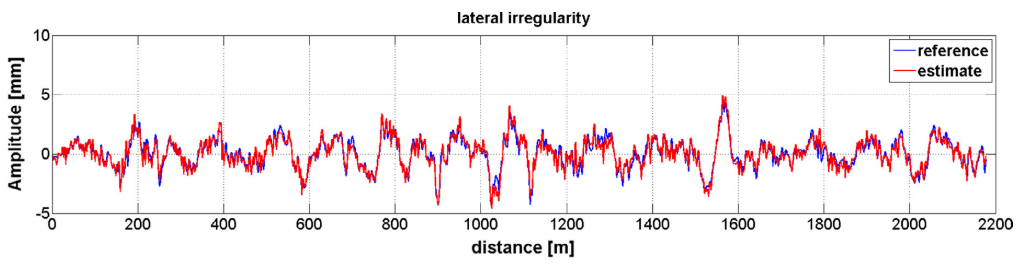
\includegraphics[width=8cm]{Cap2_LitReview/Track_Quality_Accel/DeRosa_Results_UIO.png}
%         \caption{Adapted from \cite{DEROSA2019606}}
%         \label{fig:deRosa_b}
%     \end{subfigure}
%     \\
%     \begin{subfigure}{0.8\textwidth}
%         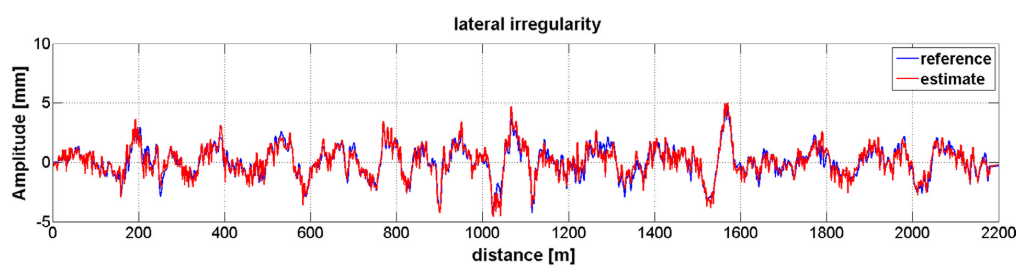
\includegraphics[width=8cm]{Cap2_LitReview/Track_Quality_Accel/DeRosa_Results_Kalman.png}
%         \caption{Adapted from \cite{DEROSA2019606}}
%         \label{fig:deRosa_c}
%     \end{subfigure}
%     \caption{Caption}
%     \label{fig:DeRosa_Results}
% \end{figure}

% \begin{table}[H]
% \centering
% \begin{tabular}{l c c c}
% \hline
%  & FD & UIO & KF \\
% \hline
% \textbf{No Noise} & & & \\
% \quad $\mathbf{J_y}$ & 0.325 & 0.291 & 0.363 \\
% \quad $\mathbf{J_p}$ & 0.122 & 0.549 & 0.124 \\
% \textbf{With Noise} & & & \\
% \quad $\mathbf{J_y}$ & 0.326 & 0.828 & 0.425 \\
% \quad $\mathbf{J_p}$ & 0.162 & 2.781 & 0.194 \\
% \hline
% \end{tabular}
% \caption{\cite{DEROSA2019606}}
% \label{table:DeRosa}
% \end{table}


\section{Identifying Track Defects Using IRVs} \label{sec-IRV-track-defect-identification}

\chapter{Methodology} \label{sec-methodology}


\chapter{Results} \label{sec-Results}

% ---
% --------------------
% FIM DOS EXEMPLOS
% --------------------
% ----------------------------------------------------------
% CONSIDERAÇÕES FINAIS
% Finaliza a parte no bookmark do PDF para que se inicie o
% bookmark na raiz e adiciona espaço de parte no Sumário
\phantompart
\chapter{Conclusion} \label{sec-conclusion}

% ----------------------------------------------------------
% ---------------------------------------------------------------------------------
% %%%%%%%%%%%%%%%%%%%%%%%%%% FIM DOS ELEMENTOS TEXTUAIS %%%%%%%%%%%%%%%%%%%%%%%%%%
% ---------------------------------------------------------------------------------
% ---------------------------------------------------------------------------------
% %%%%%%%%%%%%%%%%%%%%%%% INÍCIO DOS ELEMENTOS PÓS-TEXTUAIS %%%%%%%%%%%%%%%%%%%%%%%
% ---------------------------------------------------------------------------------
% ----------------------------------------------------------
\postextual
% ----------------------------------------------------------
% ----------------------------------------------------------
% REFERÊNCIAS
\bibliography{abntex2-modelo-references}
% ----------------------------------------------------------
% ----------------------------------------------------------
% GLOSSÁRIO
% ----------------------------------------------------------
\phantompart
\cleardoublepage
\phantomsection
\addcontentsline{toc}{chapter}{\glossaryname}
\printglossaries
% ----------------------------------------------------------
% ----------------------------------------------------------
% APÊNDICES
\begin{apendicesenv}
% Imprime uma página indicando o início dos apêndices
\partapendices
\chapter{Deriving the Backpropagationg Rule} \label{appendix-a}

TODO: Fazer a demonstracao do update dos pesos da Neural network. Usar como base \cite{Roth_2016}



%\chapter{Nullam elementum urna vel imperdiet sodales elit ipsum pharetra ligula
%c pretium ante justo a nulla curabitur tristique arcu eu metus}


\end{apendicesenv}
% ----------------------------------------------------------
% ----------------------------------------------------------
% ANEXOS
\begin{anexosenv}
% Imprime uma página indicando o início dos anexos
\partanexos
\chapter{Morbi ultrices rutrum lorem.}

\lipsum[30]

\chapter{Cras non urna sed feugiat cum sociis natoque penatibus et magnis dis
parturient montes nascetur ridiculus mus}

\lipsum[31]

\chapter{Fusce facilisis lacinia dui}

\lipsum[32]
\end{anexosenv}
% ----------------------------------------------------------
%-----------------------------------------------------------
% INDICE REMISSIVO
%-----------------------------------------------------------
\phantompart
\printindex
%-----------------------------------------------------------
% ---------------------------------------------------------------------------------
% %%%%%%%%%%%%%%%%%%%%%%%%%% FIM DOS ELEMENTOS TEXTUAIS %%%%%%%%%%%%%%%%%%%%%%%%%%
% ----------------------------------------------------------------------------------
% -----------------------------------------------------------------------------------------------
% %%%%%%%%%%%%%%%%%%%%%%%%%%%%%%%%%%%%%% FIM DO DOCUMENTO %%%%%%%%%%%%%%%%%%%%%%%%%%%%%%%%%%%%%%
% -----------------------------------------------------------------------------------------------
\end{document}